% !Mode:: "TeX:UTF-8"
%----------------------------------------------------------------------------------------
%	配置
%----------------------------------------------------------------------------------------
\documentclass[12pt]{article}
\usepackage[nofonts]{ctex}
\usepackage{graphicx}
\usepackage{amsmath}
\usepackage{cite}
\usepackage{fancyhdr}

\pagestyle{fancy}
\renewcommand{\headrule}{\hrule depth0pt height0.15truemm width\textwidth }

\rhead{
\includegraphics[width=3cm]{./images/北京航空航天大学logo.png}}
\lhead{\bfseries 主动消振文档} 

\usepackage[document]{ragged2e}
\usepackage[skip=2pt]{caption}
\usepackage{float}
%use for mac
\setCJKmainfont[BoldFont=STHeiti,ItalicFont=STKaiti]{STSong}
%use for windows
%\setCJKmainfont[BoldFont=SimHei,ItalicFont=KaiTi]{SimSun}
\usepackage{tikz}
\usepackage{geometry}
\geometry{a4paper}
\linespread{1.2}
\setcounter{page}{-1}

\begin{document}

\tikz[remember picture,overlay] \node[opacity=1.0,inner sep=0pt] at (current page.center){
\includegraphics[width=\paperwidth,height=\paperheight]{./images/background.pdf}};
\vskip 4.5in

%----------------------------------------------------------------------------------------
%	首页
%----------------------------------------------------------------------------------------
\thispagestyle{empty}
\begin{center}
{\Huge\textbf{
%% -----> 此处修改题目 <----- %%
双边溢流自适应陷波算法分析
%% -----> 题目修改完毕 <----- %%
}}
\newline
\vskip 0.3in
\end{center}
\begin{flushright}
{\LARGE{
%% -----> 此处修改作者 <----- %%
郑慧伟
%% -----> 作者修改完毕 <----- %%
}}
\newline
\vskip 2in
{\Large{
%% -----> 此处修改时间 <----- %%
2017年03月31日
%% -----> 修改时间完毕 <----- %%
}}
\end{flushright}
\clearpage


%----------------------------------------------------------------------------------------
%	目录页
%----------------------------------------------------------------------------------------
\tableofcontents
\thispagestyle{empty}
\newpage

%----------------------------------------------------------------------------------------
%	正文
%----------------------------------------------------------------------------------------
\section{概述}
\label{sec:sec1}
一维流体波动的振动信号,从时域的角度来看,就是多谐波信号和干扰信号的叠加。消振的目的,就是对振动信号中的基频率信号以及相应的倍频信号进行消除。
\vspace{3mm}
\par
主动消振,是指针对特定的待消除的目标信号,采用人为生成的频率相同,相位相反的激励信号,施加到原始振动信号上,使得原始信号和激励信号进行干涉,最终消除原始波动的整套方案。如何生成激励信号,以及如何将激信号按要求施加到原始振动信号上,是主动消振算法的两大核心问题。前者称为构建控制器算法,后者称为次级通道辨识/建模方法。
\vspace{3mm}
\par
主动消振构建控制器的方法不计其数,但核心问题就是如何针对目标信号构建频率相同,相位相反的激励信号。从建模的角度来看,就是针对信号源进行了一次辨识,人为地构建了一个和信号源互斥的信号发生器,可以产生与信号源频率相同,相位相反的信号。这里采用的是自适应陷波算法。
\vspace{3mm}
\par
次级通道辨识/建模方法,是描述如何将激励信号按要求等量纲的施加到原始振动信号上,尽可能地减少频率、相位和幅值的损失。举个简单例子,在实际控制系统中,人为生成的激励信号是计算机数字信号,经过DA输出变成模拟电信号,然而模拟电信号和真实的振动信号不能直接叠加,需要经过特定的执行器,将电信号转化为与振动信号等量纲的信号(比如液压的溢流流量信号),从而完成信号的叠加和消振。从控制器输出的电信号到具体的执行器输出的执行信号之间,存在一个变换关系,如何得到该变换关系的方法,称为次级通道辨识或建模方法。辨识,是数据驱动的方法,是指建立变换关系的模型,计算机不断采集输入输出信号,对变换关系进行自动建模。建模,是知识驱动的方法,人为知道执行器的一些物体特性,按照物体及数学推导,人为建立输出和输出之间的变换关系。

\section{自适应陷波算法}
自适应滤波算法框架,是目前解决振动消除问题的最成熟算法框架。按控制信号流来分,可以分为前馈和反馈两类算法。按待消除的信号频率带宽来分,可以分为宽频消振和窄频消振。经过简单组合,从大的方向上来说,就存在四类算法,分别是自适应前馈宽频消振算法,自适应前馈窄频消振算法,自适应反馈宽频消振算法,自适应反馈窄频消振算法。自适应陷波算法(Active Notch Filter),隶属于自适应前馈窄频消振算法。

\subsection{原理}
图\ref{fig:fig1}是自适应陷波算法方案图。算法的核心分2部分,第一部分是信号发生器,目的是人为构建参考信号,从而可以让自适应陷波算法可以融入自适应滤波算法框架中;第二部分是LMS算法优化部分,通过不断迭代优化信号发生器的参数,使得信号发生器可以真实的模拟原始信号,达到建模的目的。
\begin{figure}[H]
\begin{center}
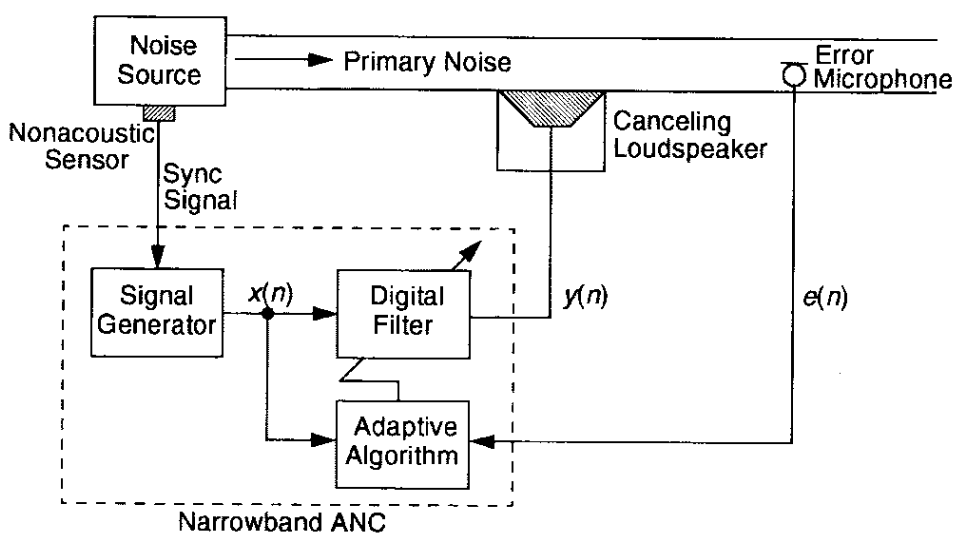
\includegraphics[width=0.9\linewidth]{./images/自适应陷波滤波原理草图.png}
\caption{自适应陷波滤波方案图}
\label{fig:fig1}
\end{center}
\end{figure}

先从最基本的自适应陷波器开始介绍,为了简洁起见,这里我们不计次级通道的影响。图\ref{fig:fig2} 是自适应陷波滤波器的原理图。自适应陷波的核心是陷波器,所谓陷波器,就是对某一特定频率的信号进行消除,所以陷波器的本质是构建一个与待消频率一致的正弦信号,使得相位与原始信号相反。幅值和频率都可以相对简单的获取,现在的核心问题是如何精确地构建这个消振信号的相位。陷波器的思想是三角函数的全角公式。

\begin{figure}[H]
\begin{center}
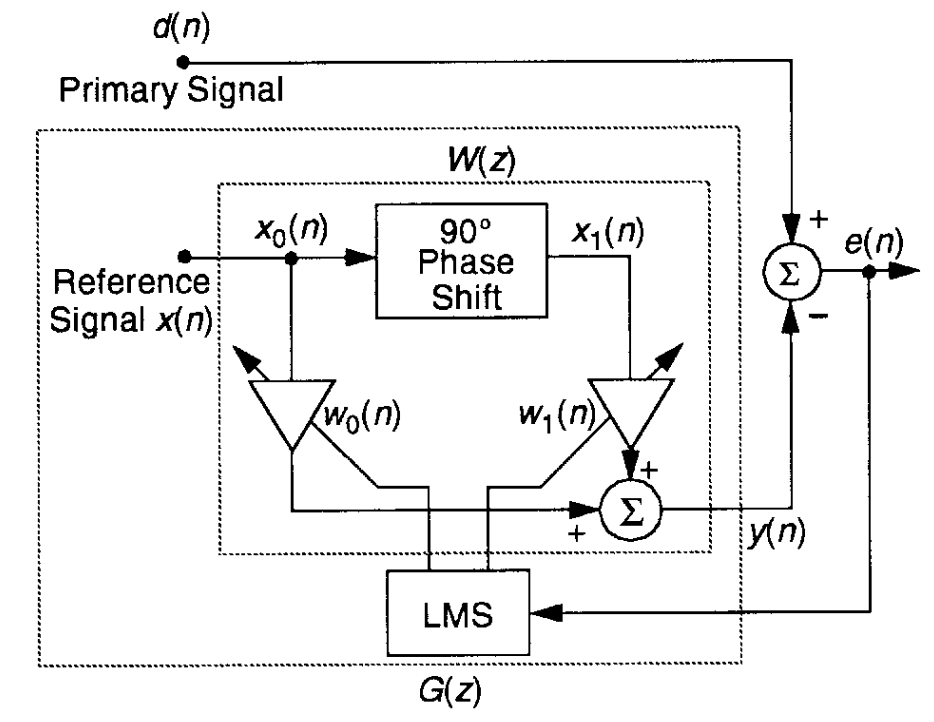
\includegraphics[width=0.9\linewidth]{./images/自适应陷波滤波器原理.png}
\caption{自适应陷波滤波器原理图}
\label{fig:fig2}
\end{center}
\end{figure}

对原始信号进行傅里叶变换,得到待消信号的频率$f$ 。人为构建参考信号输入源$x_{0}(n)=A\cos(2\pi fn)$,其中$A$和$f$是参考信号的幅值和频率。对$x_{0}(n)$做$90^{\circ}$的相位偏移,得到另外一个参考信号输入源$x_{1}(n)=A\sin(2\pi fn)$,于是我们可以得到参考信号为:

\begin{align}
x_{ref} &= \omega_{0}x_{0}(n)+\omega_{1}x_{1}(n)  \nonumber \\
&= \omega_{0}A\cos(2\pi fn)+\omega_{1}A\sin(2\pi fn)
\end{align}

利用三角函数全角公式进行推导:

\begin{align}
x_{ref} &= \omega_{0}A\cos(2\pi fn)+\omega_{1}A\sin(2\pi fn) \nonumber \\
&=A\sqrt{\omega_{0}^{2}+\omega_{1}^{2}}\left(\frac{\omega_{0}}{\sqrt{\omega_{0}^{2}+\omega_{1}^{2}}}\cos(2\pi fn)+\frac{\omega_{1}}{\sqrt{\omega_{0}^{2}+\omega_{1}^{2}}}\sin(2\pi fn)\right) \nonumber \\
&=A\sqrt{\omega_{0}^{2}+\omega_{1}^{2}}\sin(2\pi fn+\psi) \\
&\mbox{其中}  \psi = \arctan\frac{\omega_{0}}{\omega_{1}} \nonumber
\end{align}

所以只要改变$\omega_{0}$和$\omega_{1}$的值,就可以相应改变相位差$\psi$的值,实现相位的优化。

利用LMS优化算法迭代推导,可以得到权系数优化规则为:

\begin{align}
\omega_{0}(n+1)=\omega_{0}(n) + \mu e(n)x_{0}(n) \nonumber \\
\omega_{1}(n+1)=\omega_{1}(n) + \mu e(n)x_{1}(n)
\end{align}

如果将次级通道简化为一个纯延时环节,那么可以得到优化方程为:

\begin{align}
\omega_{0}(n+1)=\omega_{0}(n) + \mu e(n)x_{0}(n-\Delta) \nonumber \\
\omega_{1}(n+1)=\omega_{1}(n) + \mu e(n)x_{1}(n-\Delta) 
\end{align}

其中$\Delta$是次级通道的延时系数,需要通过实验人为整定。

再进一步,考虑实际情况,次级通道是一个传递函数$S(z)$,假设我们通过次级通道辨识算法得到了次级通路的估计$\hat{S}(z)$,那么我们可以得到我们的优化方程为:

\begin{align}
\omega_{0}(n+1)=\omega_{0}(n) + \mu e(n)x^{\prime}_{0}(n) \nonumber \\
\omega_{1}(n+1)=\omega_{1}(n) + \mu e(n)x^{\prime}_{1}(n) 
\end{align}
其中$x^{\prime}_{0}(n)$和$x^{\prime}_{1}(n)$是$x_{0}(n)$和$x_{1}(n)$经过估计的次级通路$\hat{S}(z)$滤波后的输出,从时域上来看是$\hat{S}(z)$的拉普拉斯反变换分别和$x_{0}(n)$、$x_{1}(n)$的卷积。

图\ref{fig:fig3}是考虑次级通路的自适应陷波LMS算法原理图。

\begin{figure}[H]
\begin{center}
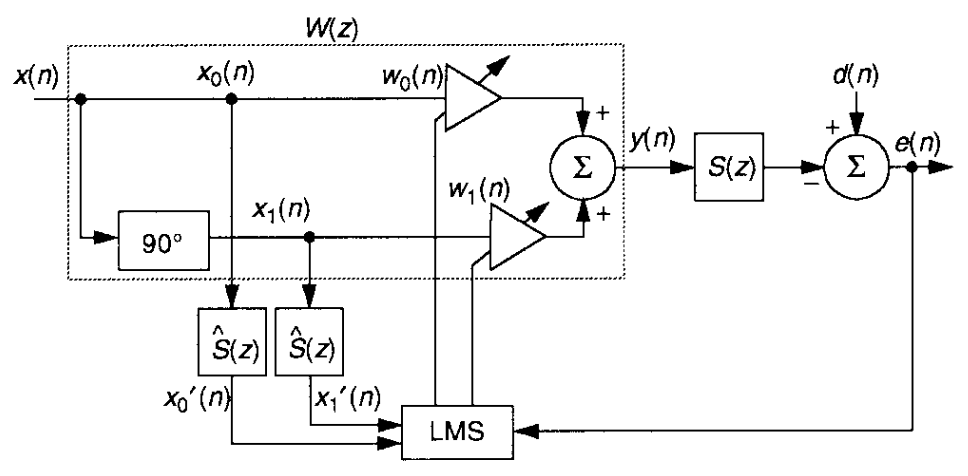
\includegraphics[width=0.9\linewidth]{./images/自适应陷波LMS算法原理图.png}
\caption{自适应陷波LMS算法原理图}
\label{fig:fig3}
\end{center}
\end{figure}

\subsection{优点}
从原始输入$d(n)$到误差信号输出$e(n)$的传递函数$H(z)$为\cite{widrow1975adaptive}:

\begin{align}
H(z)=\frac{z^{2}-2z\cos2\pi f+1}{z^{2}-(2-\frac{\mu LA^{2}}{2})z\cos2\pi f+1-\frac{\mu LA^{2}}{2}}
\end{align}

$L$是陷波器的阶数,在我们的情况下,$L=2$。

自适应陷波算法的$-3dB$带宽为\cite{glover1977adaptive}:

\begin{align}
B\approx\frac{\mu LA^{2}}{4\pi T}=\frac{\mu A^{2}}{2\pi T}
\end{align}

可见优化系数$\mu$和控制信号的幅值$A$越大,对频率的容忍越大。该算法对频率不匹配有一定的容忍性。
当然,优化系数$\mu$越大,算法越不稳定,具体$\mu$的取值是一个视具体情况而折衷的一个值。

更有价值的是,自适应陷波算法对相位也有一定的抗干扰性\cite{kuo1995active}:

\begin{align}
-90^{\circ}<\phi\Delta<90^{\circ}
\end{align}

只要参考输出的相位$\psi$和原始信号的相位$\psi_{0}$之差$\phi\Delta$控制在$-90^{\circ}$和$90^{\circ}$之间,算法就可以实现消振。

\section{双边溢流原理}
双边溢流压电陶瓷伺服阀,是高带宽的压电陶瓷直驱式伺服阀,最大行程59.3$\mu$m,最大频宽700hz,空载流量达到4.45l/min。
双边溢流阀的溢流原理图如图\ref{fig:fig4}所示。

\begin{figure}[H]
\begin{center}
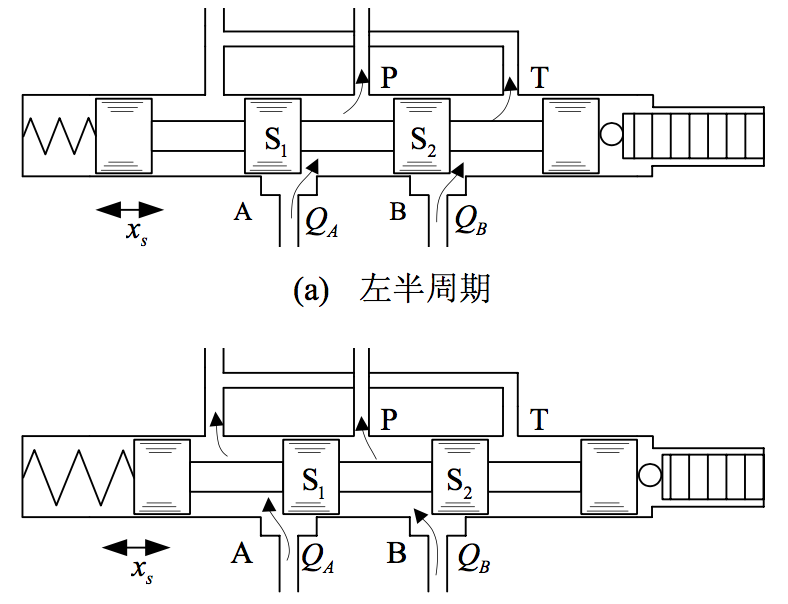
\includegraphics[width=0.9\linewidth]{./images/双边溢流阀原理图.png}
\caption{双边溢流阀原理图}
\label{fig:fig4}
\end{center}
\end{figure}

只要阀芯不在中位,不管阀芯左移还是右移,都产生一致的溢流流量,所以从数学的角度,阀芯流量流量和阀芯位移的绝对值成正比。一旦牵涉到绝对值运算,意味着双边溢流阀的传递函数是一个非线性函数。

\section{次级通道建模}
为了逼近该非线性函数,需要对次级通道进行建模。

\begin{figure}[H]
\begin{center}
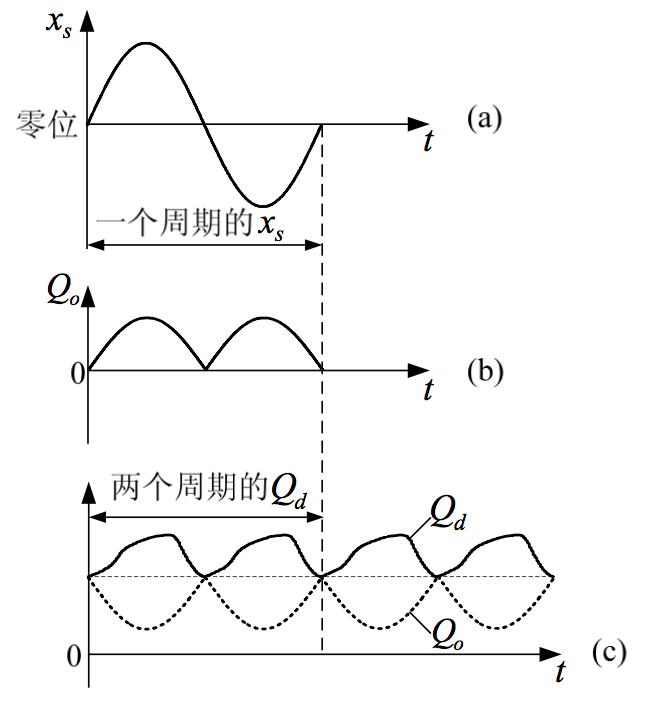
\includegraphics[width=0.9\linewidth]{./images/阀芯位移与溢流流量的频率对应图.png}
\caption{阀芯位移与溢流流量的频率对应图}
\label{fig:fig5}
\end{center}
\end{figure}

图\ref{fig:fig5}是阀芯位移与溢流流量的频率对应图,从图\ref{fig:fig5}:c可以看出,溢流流量不是一个线性函数,但可以用一个半频率的周期性正弦函数进行近似拟合,这也就是双边溢流的精髓所在。
可以推导得到半频率控制信号的相位$\theta$和原始信号的相位$\psi$直接的对应表达式:
\begin{align}
\theta = \frac{\psi}{2}+\frac{\pi}{4}
\end{align}

图\ref{fig:fig6}是两者对应关系的仿真图,可见在误差允许的情况下,用一个半频率的周期性正弦函数去近似拟合非线性的溢流流量,从原理上来说是可行的。

\begin{figure}[H]
\begin{center}
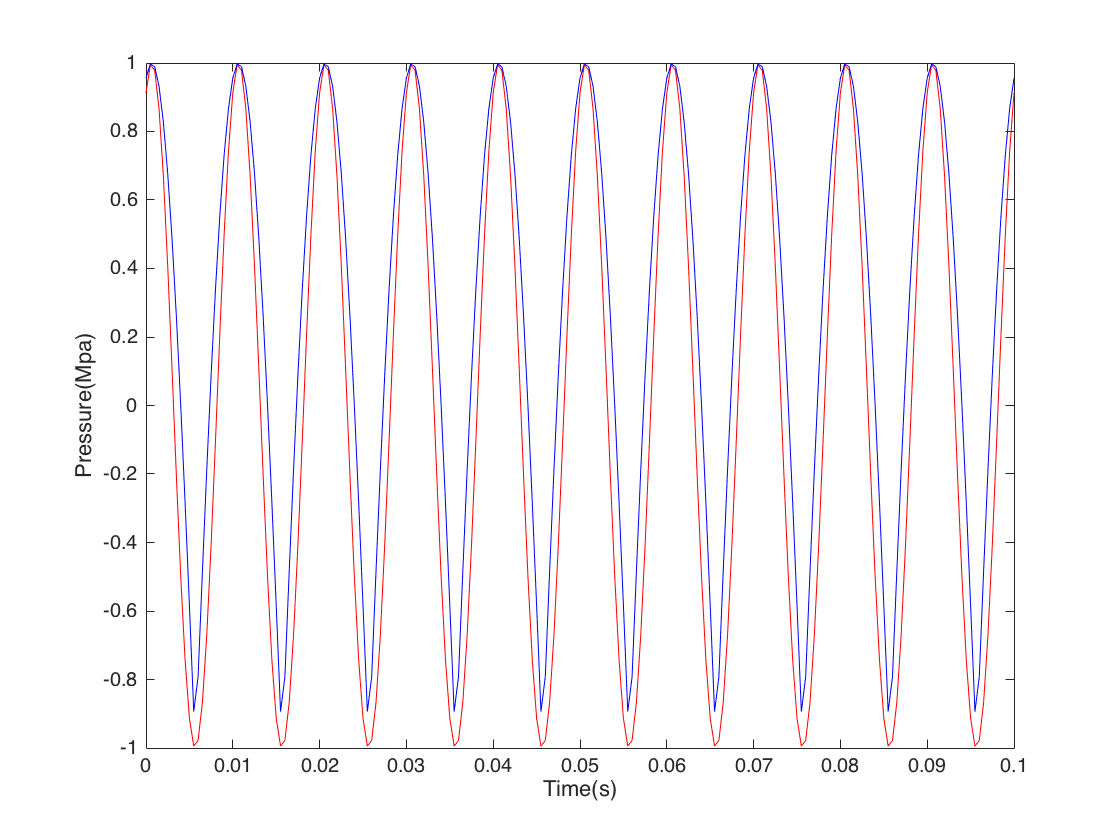
\includegraphics[width=0.9\linewidth]{./images/双边溢流相位推导演示图.png}
\caption{双边溢流相位推导演示图}
\label{fig:fig6}
\end{center}
\end{figure}

\section{实验结果}
在南京609机电液压中心进行了主动消振实验,下面进行实验结果分析。

\subsection{总体概况}
如图\ref{fig:fig7}所示,蓝色曲线为系统采集的泵出口压力,红色部分为采集回来的阀芯电位,等价于阀芯位移,可明显看出施加控制对泵出口压力有明显的消振作用。
\begin{figure}[H]
\begin{center}
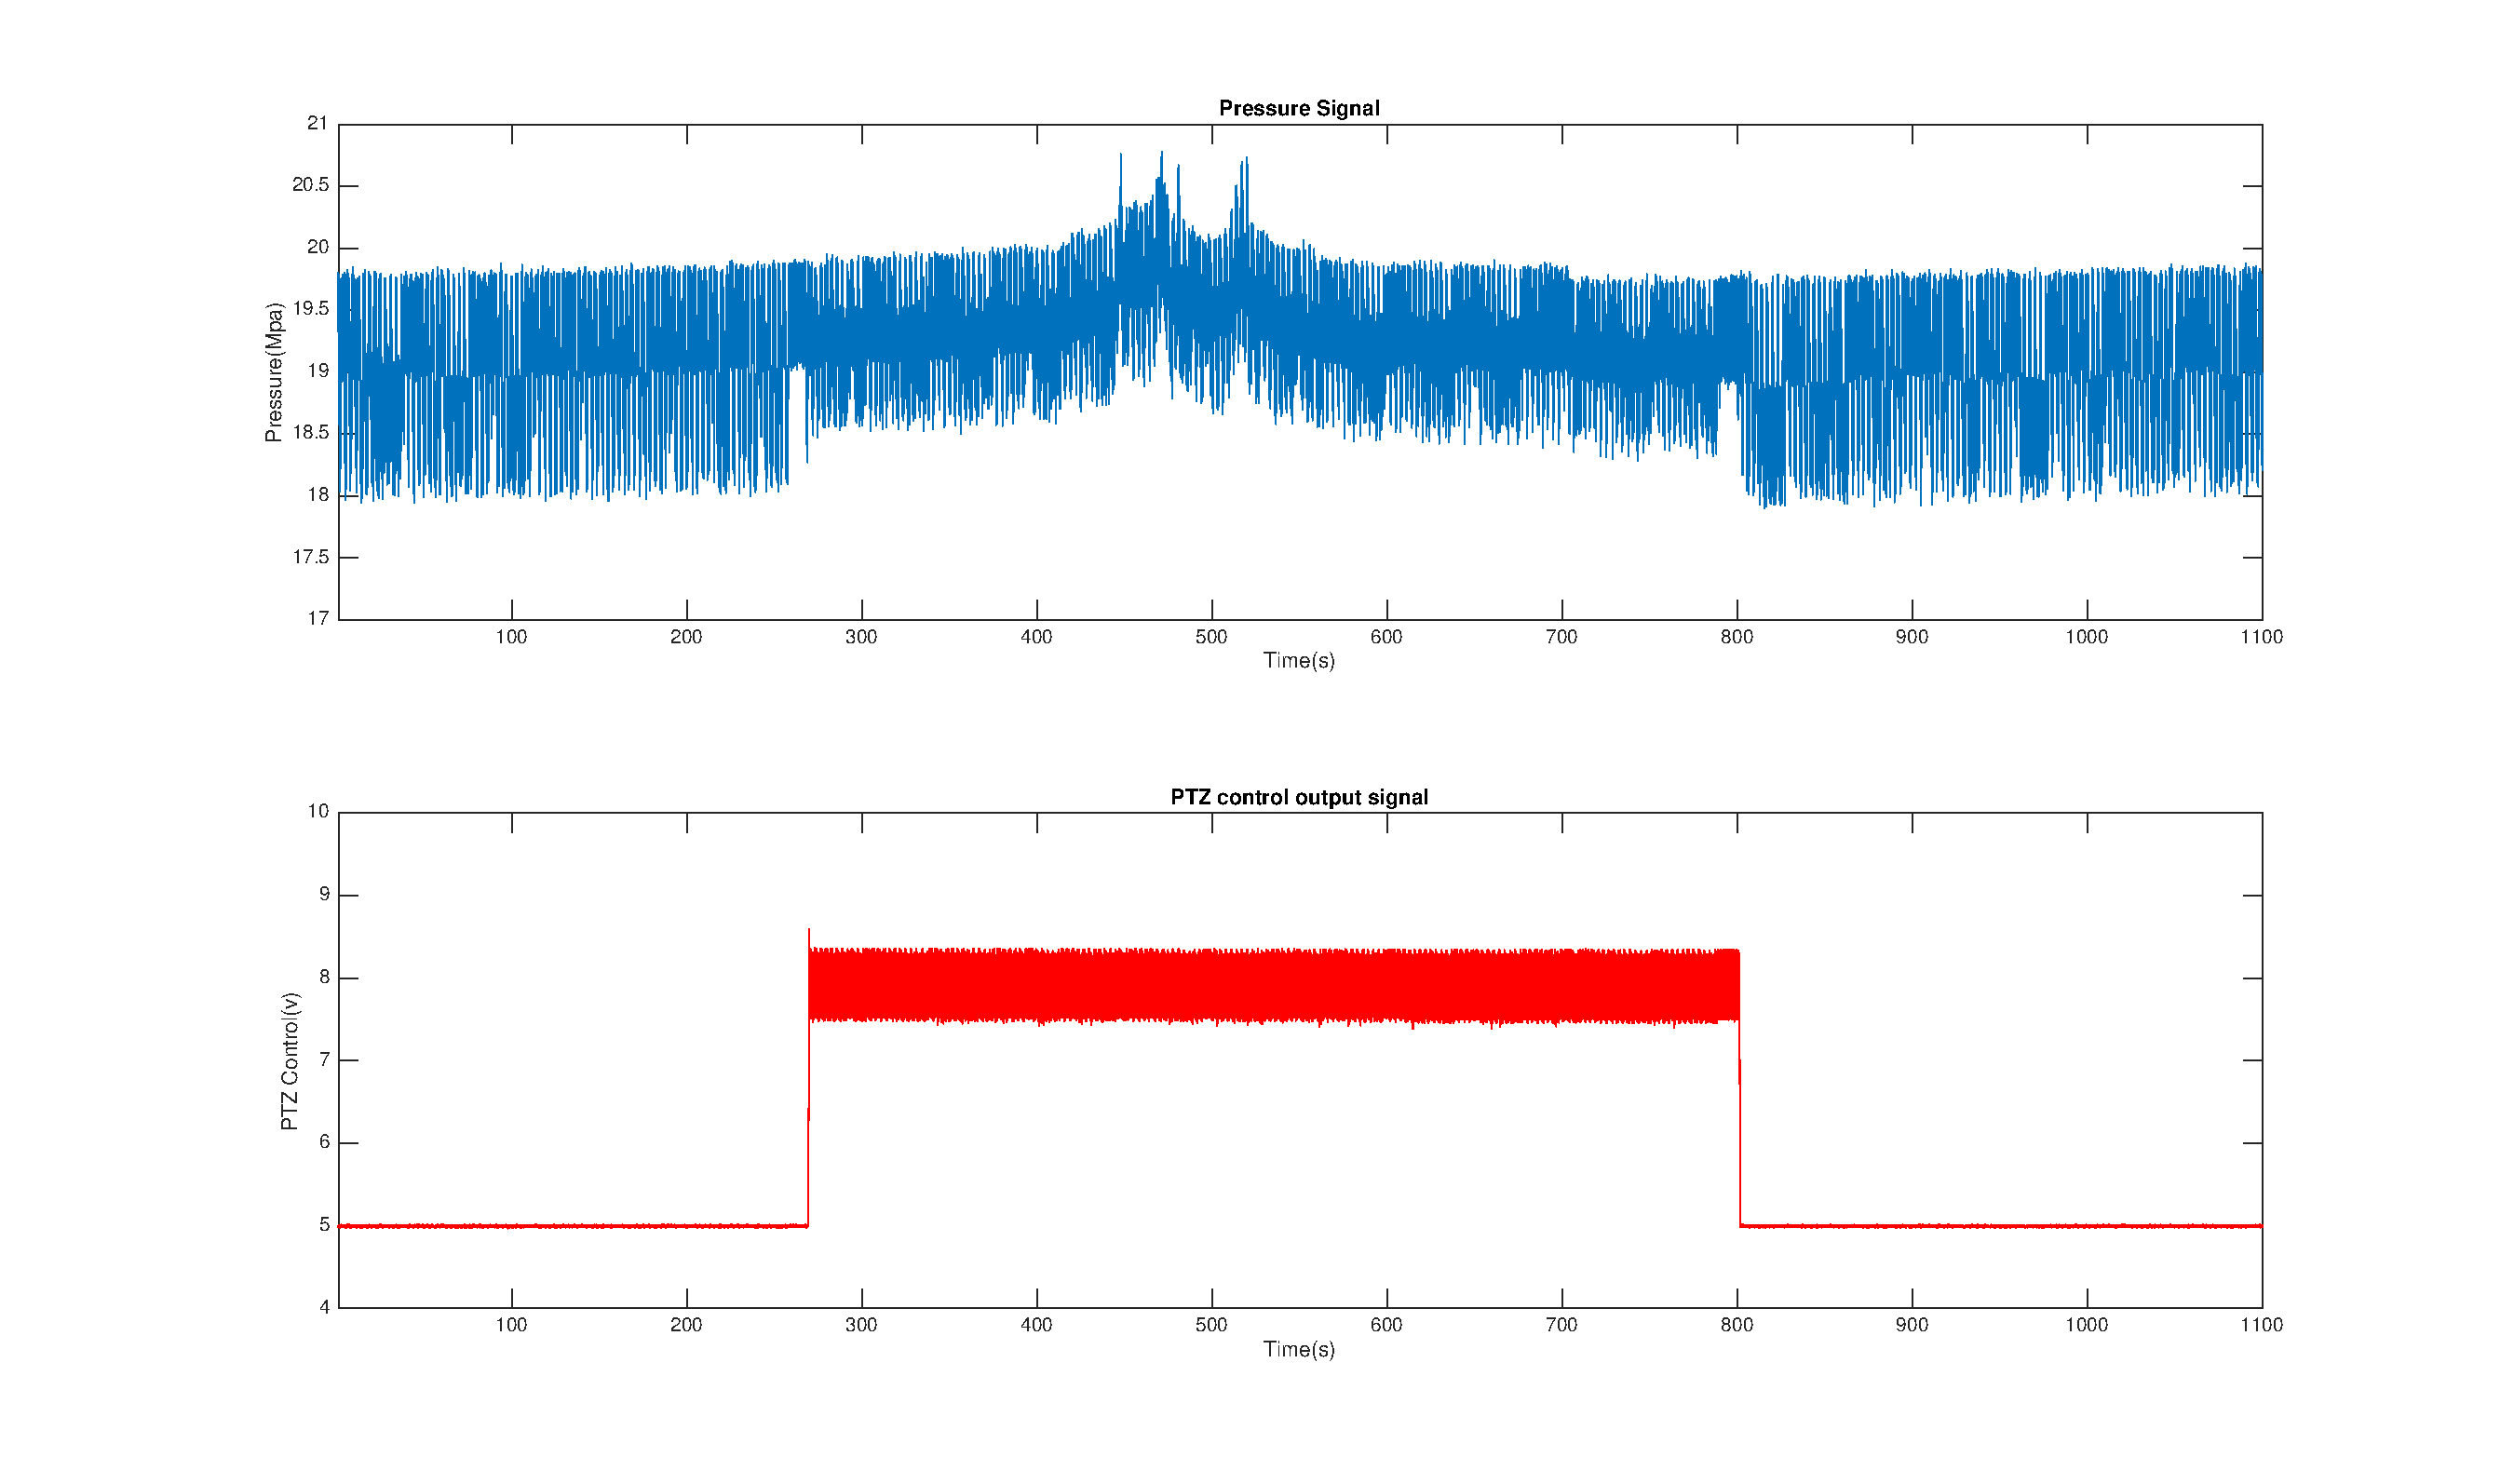
\includegraphics[width=0.9\linewidth]{./images/time_domain_overall.eps}
\caption{流体脉动主动消振总体实验效果图}
\label{fig:fig7}
\end{center}
\end{figure}

\subsection{控制之前时域频率分析}

\begin{figure}[H]
\begin{center}
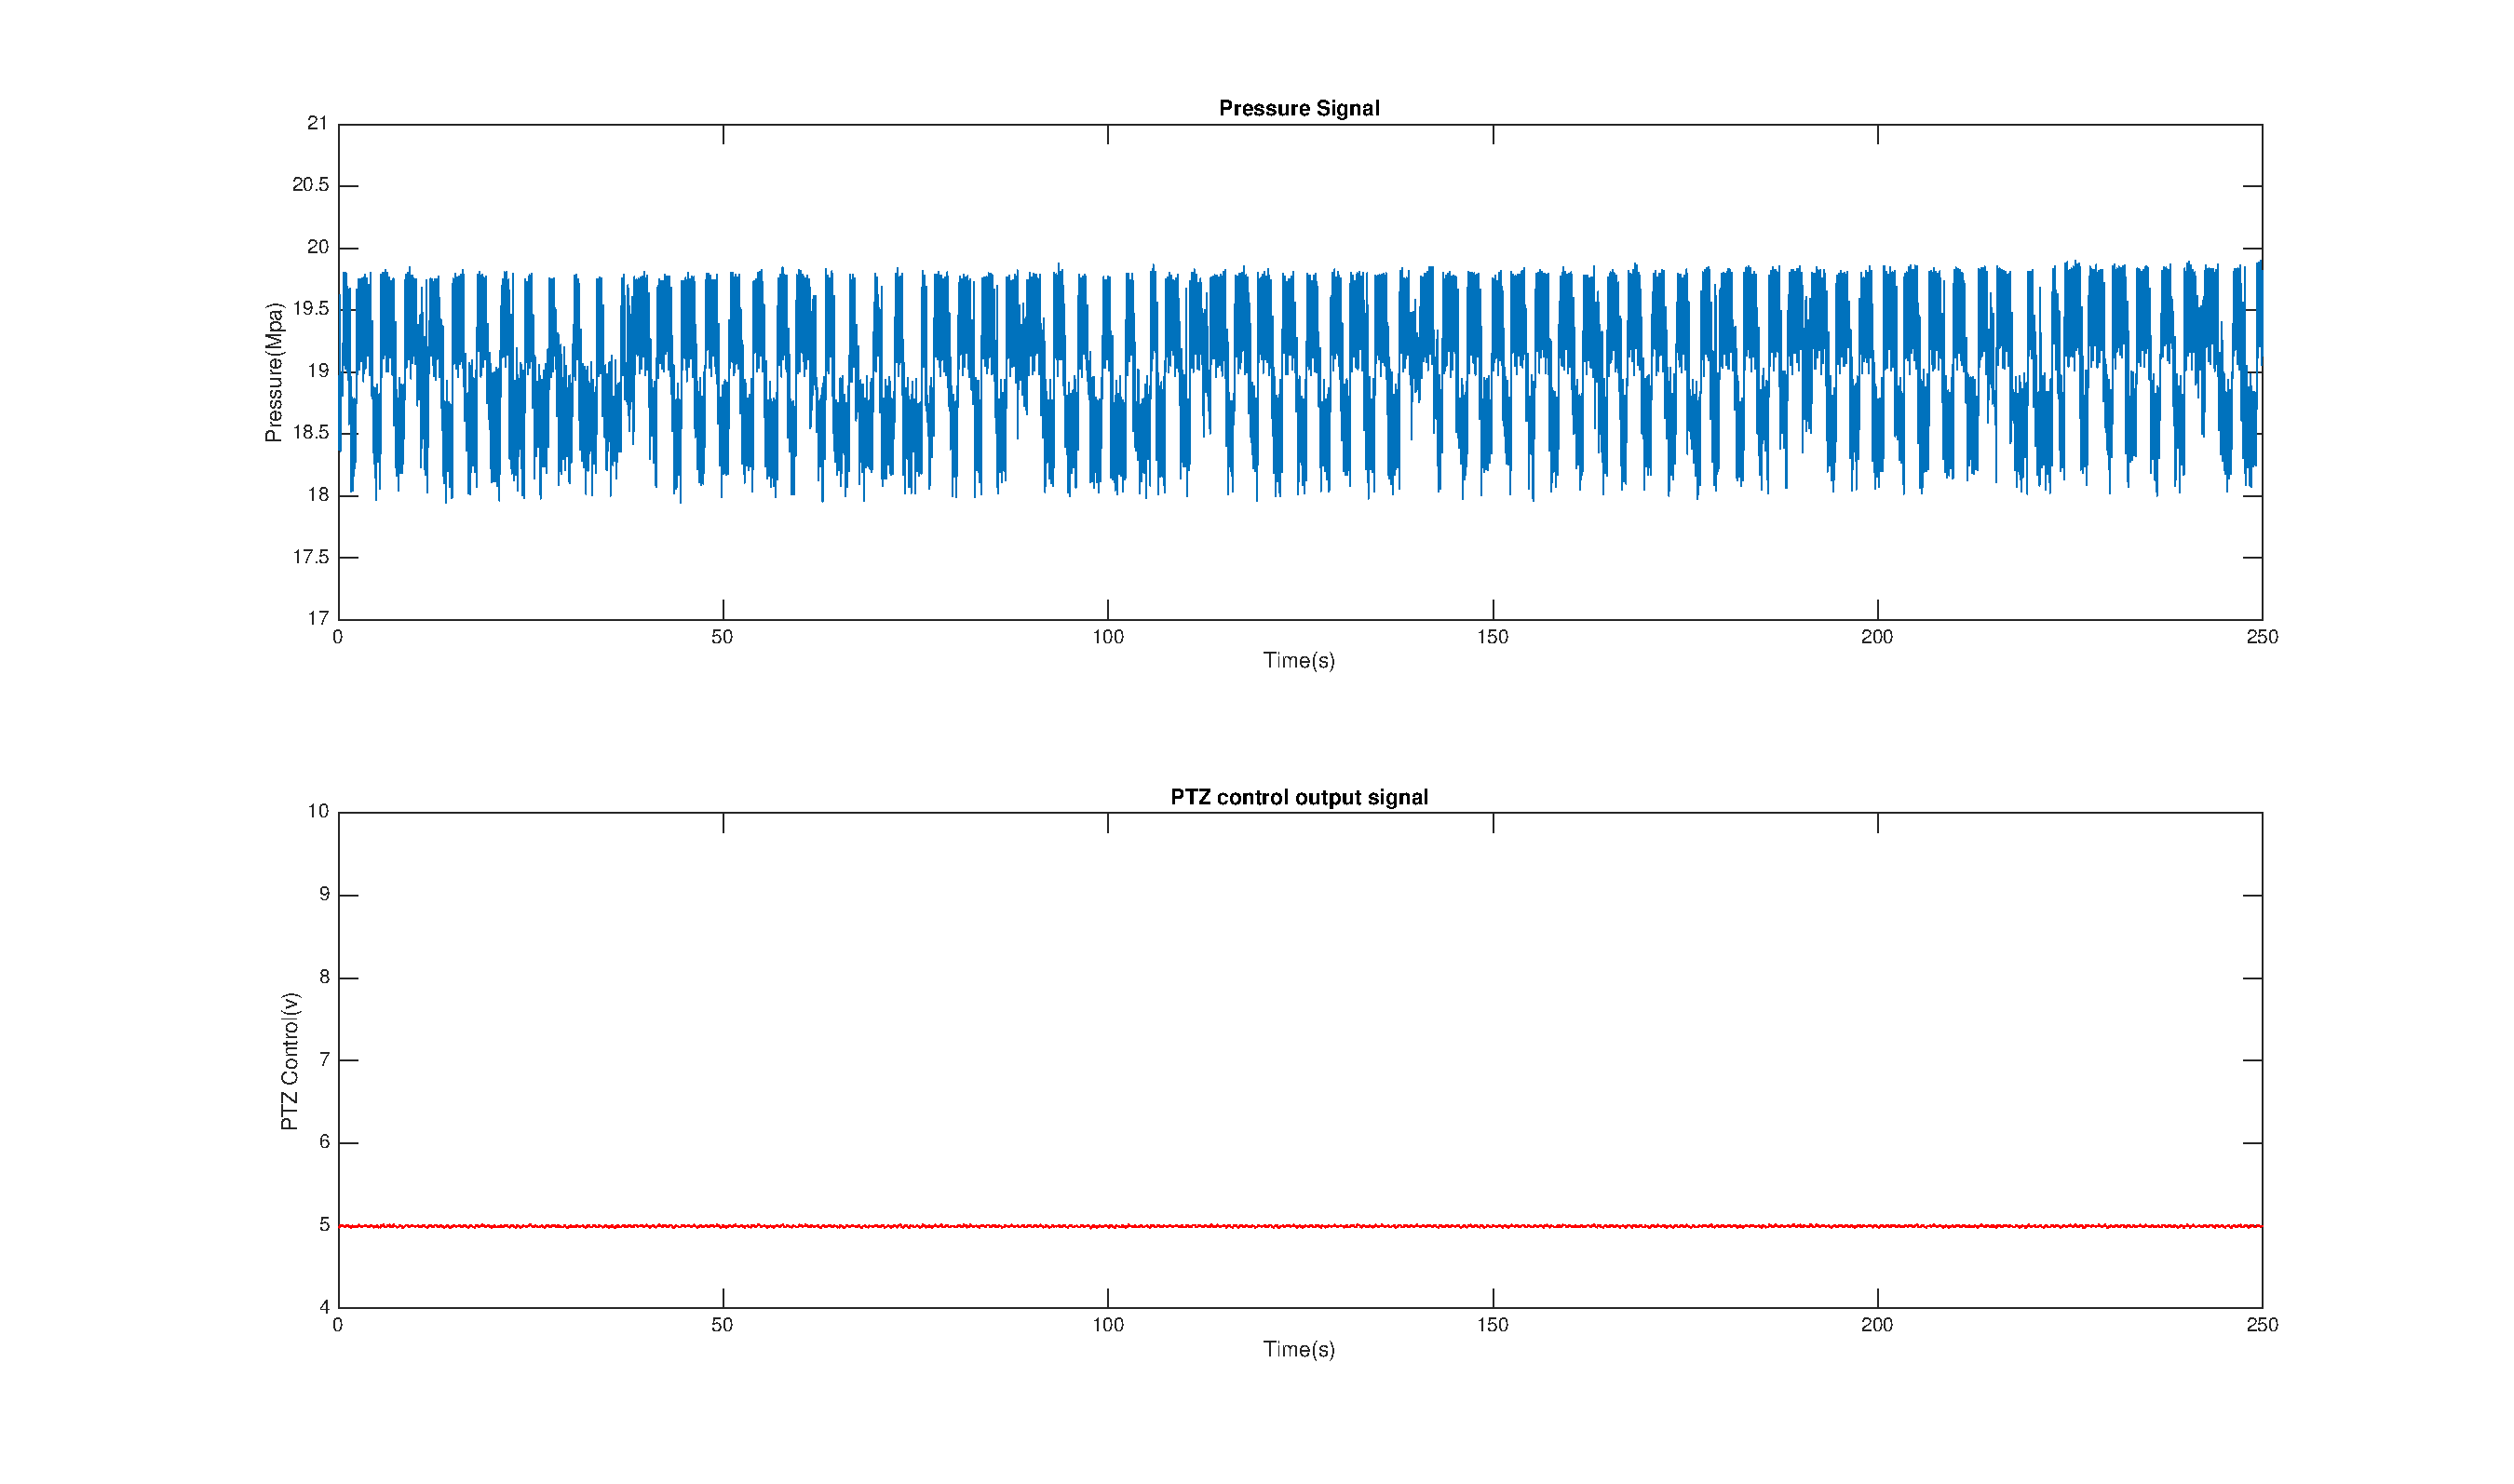
\includegraphics[width=0.9\linewidth]{./images/time_domain_result_before_control.eps}
\caption{控制之前压力脉动时域图}
\label{fig:fig8}
\end{center}
\end{figure}

\begin{figure}[H]
\begin{center}
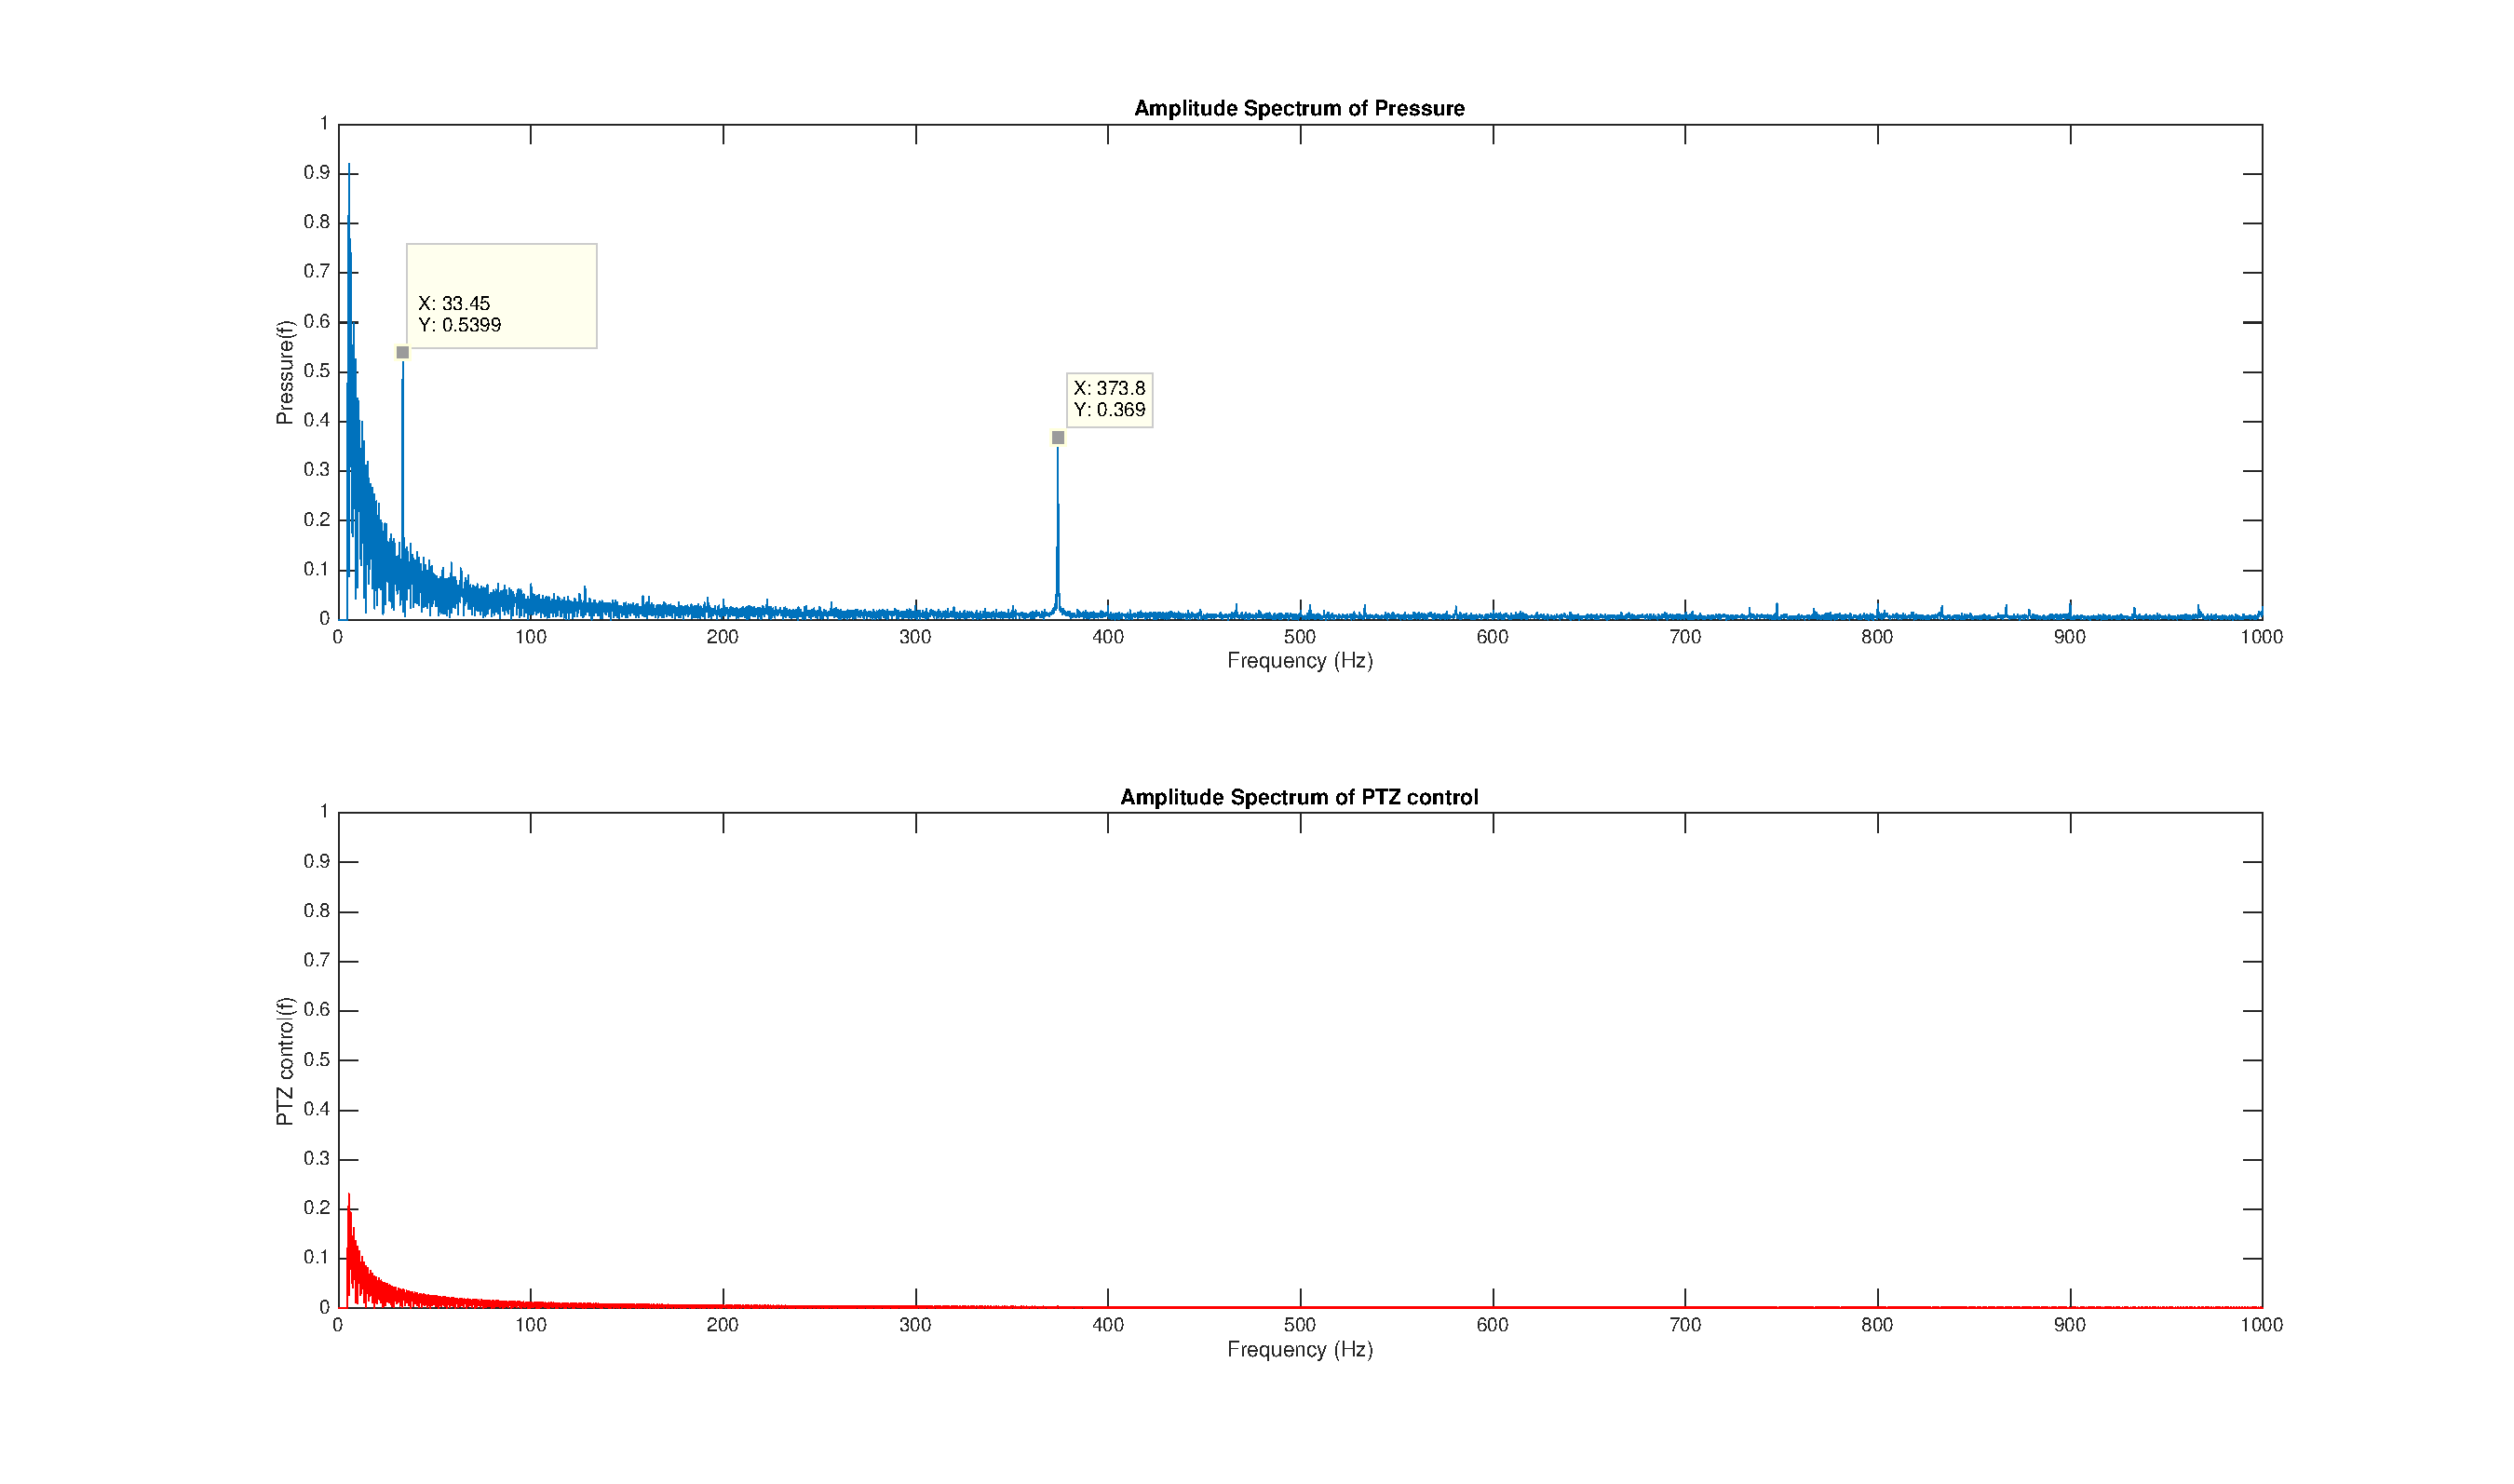
\includegraphics[width=0.9\linewidth]{./images/fft_result_before_control.eps}
\caption{控制之前压力脉动频域图}
\label{fig:fig9}
\end{center}
\end{figure}

如图\ref{fig:fig8}、图\ref{fig:fig9}所示,主要脉动频率在373.8hz,幅值为0.369Mpa,此时泵工作在2500r/min附近,理论频率为375hz,实验频率与理论频率相符。

\subsection{施加控制时域频率分析}

\begin{figure}[H]
\begin{center}
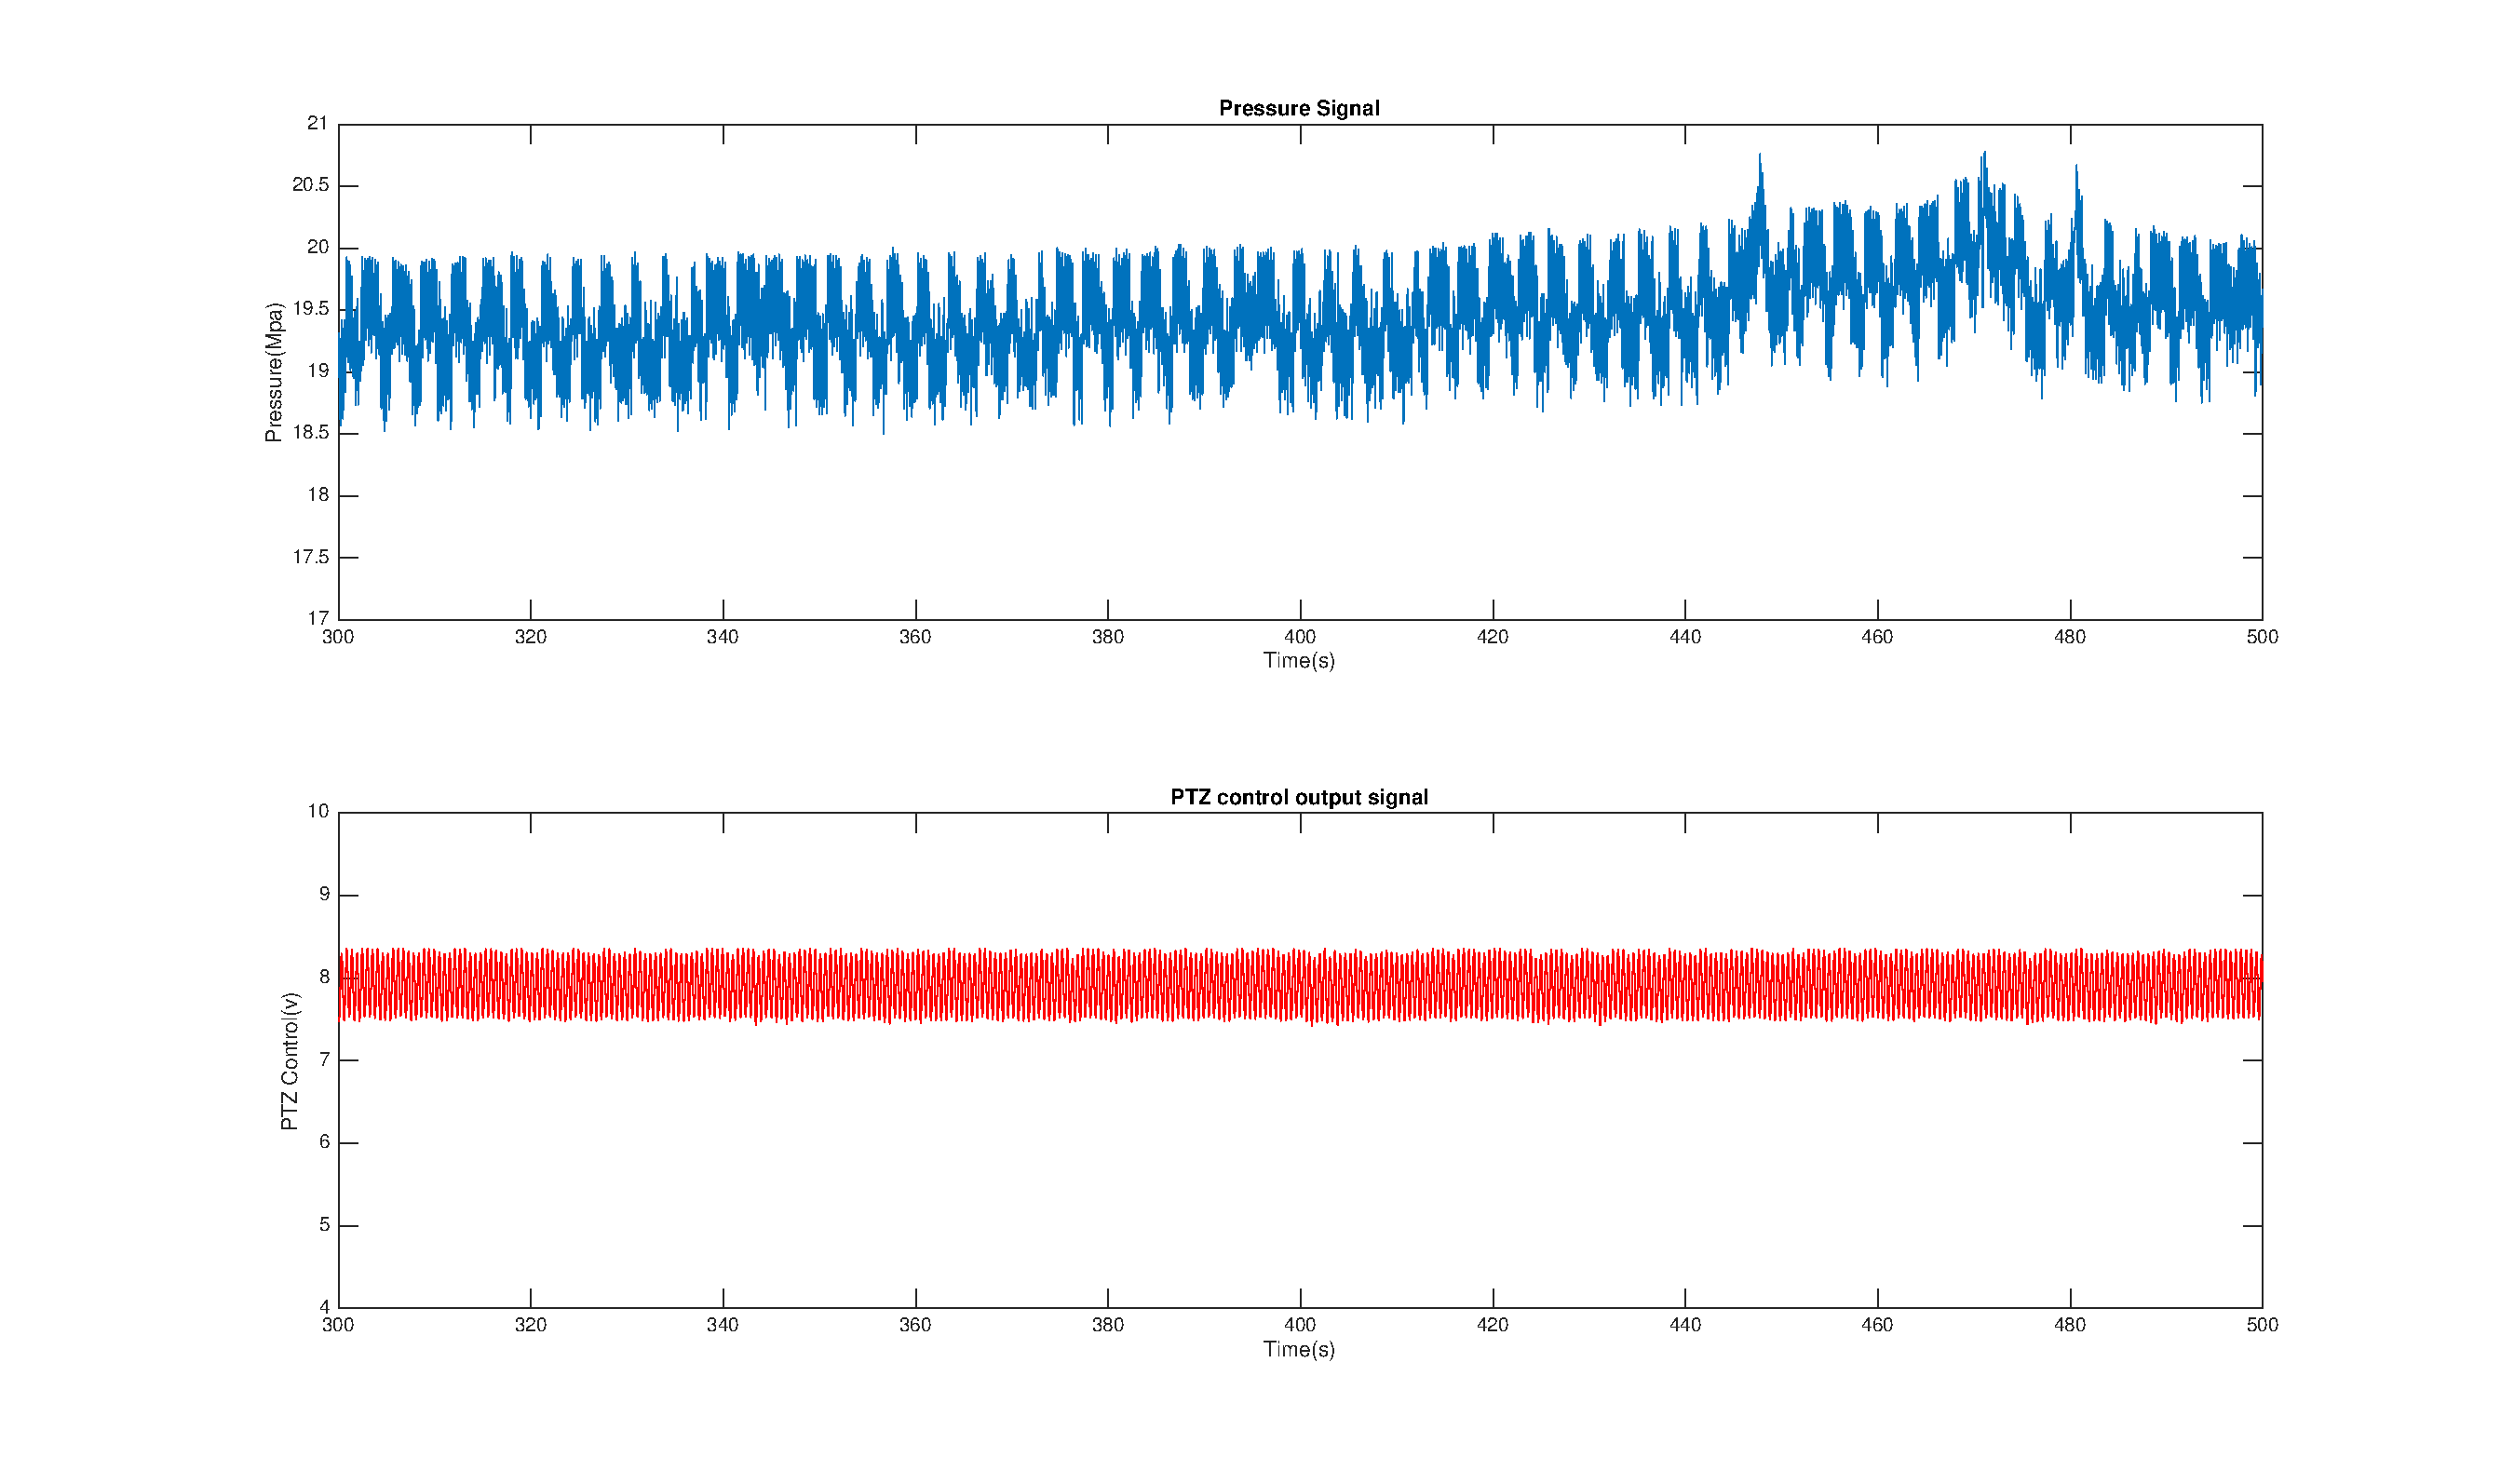
\includegraphics[width=0.9\linewidth]{./images/time_domain_result_controling.eps}
\caption{施加控制压力脉动时域图}
\label{fig:fig10}
\end{center}
\end{figure}

\begin{figure}[H]
\begin{center}
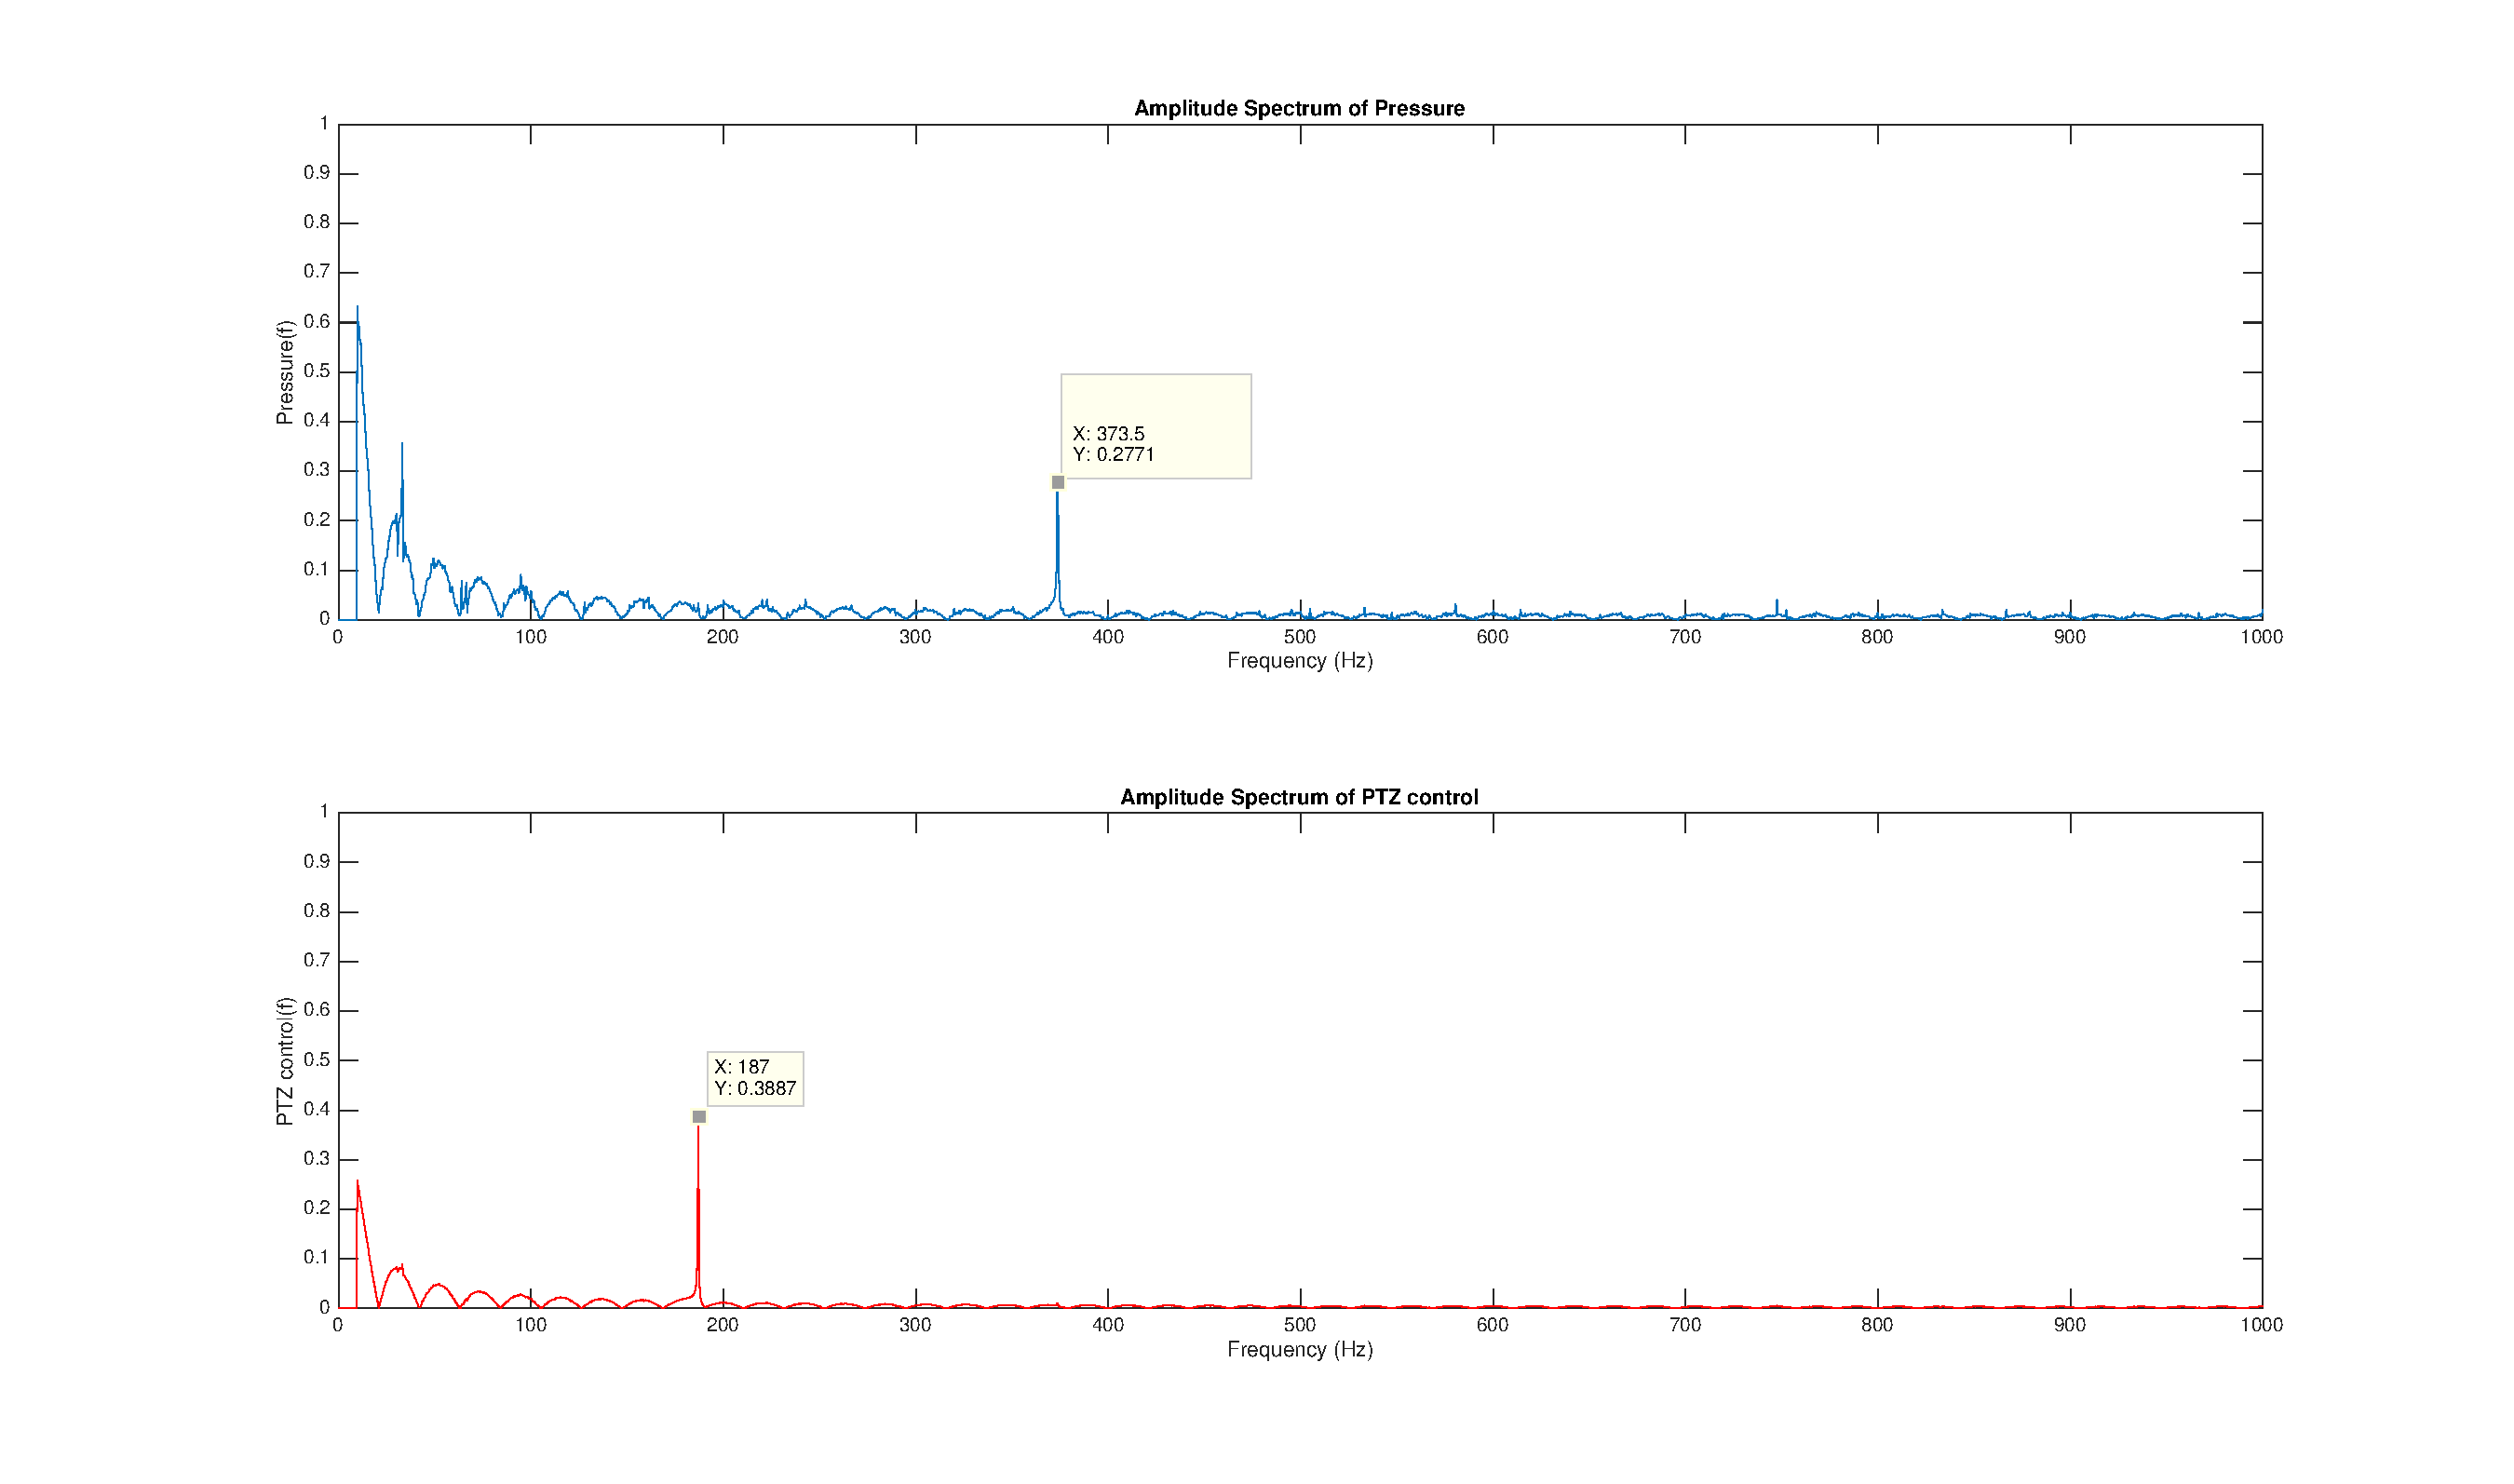
\includegraphics[width=0.9\linewidth]{./images/fft_result_controling.eps}
\caption{施加控制压力脉动频域图}
\label{fig:fig11}
\end{center}
\end{figure}

如图\ref{fig:fig10}、图\ref{fig:fig11}所示,泵脉动频率在373.5hz,双边溢流阀控制频率为187hz,基本上是泵脉动频率的一半。此时泵脉动是0.2771Mpa,比原始脉动小了很多,单从单频率消振分析,消振比例达到了25\%,从时域上来分析,在全频率范围消振比例高于单频率消振,达到38\%。

\subsection{停止控制之后时域频率分析}

\begin{figure}[H]
\begin{center}
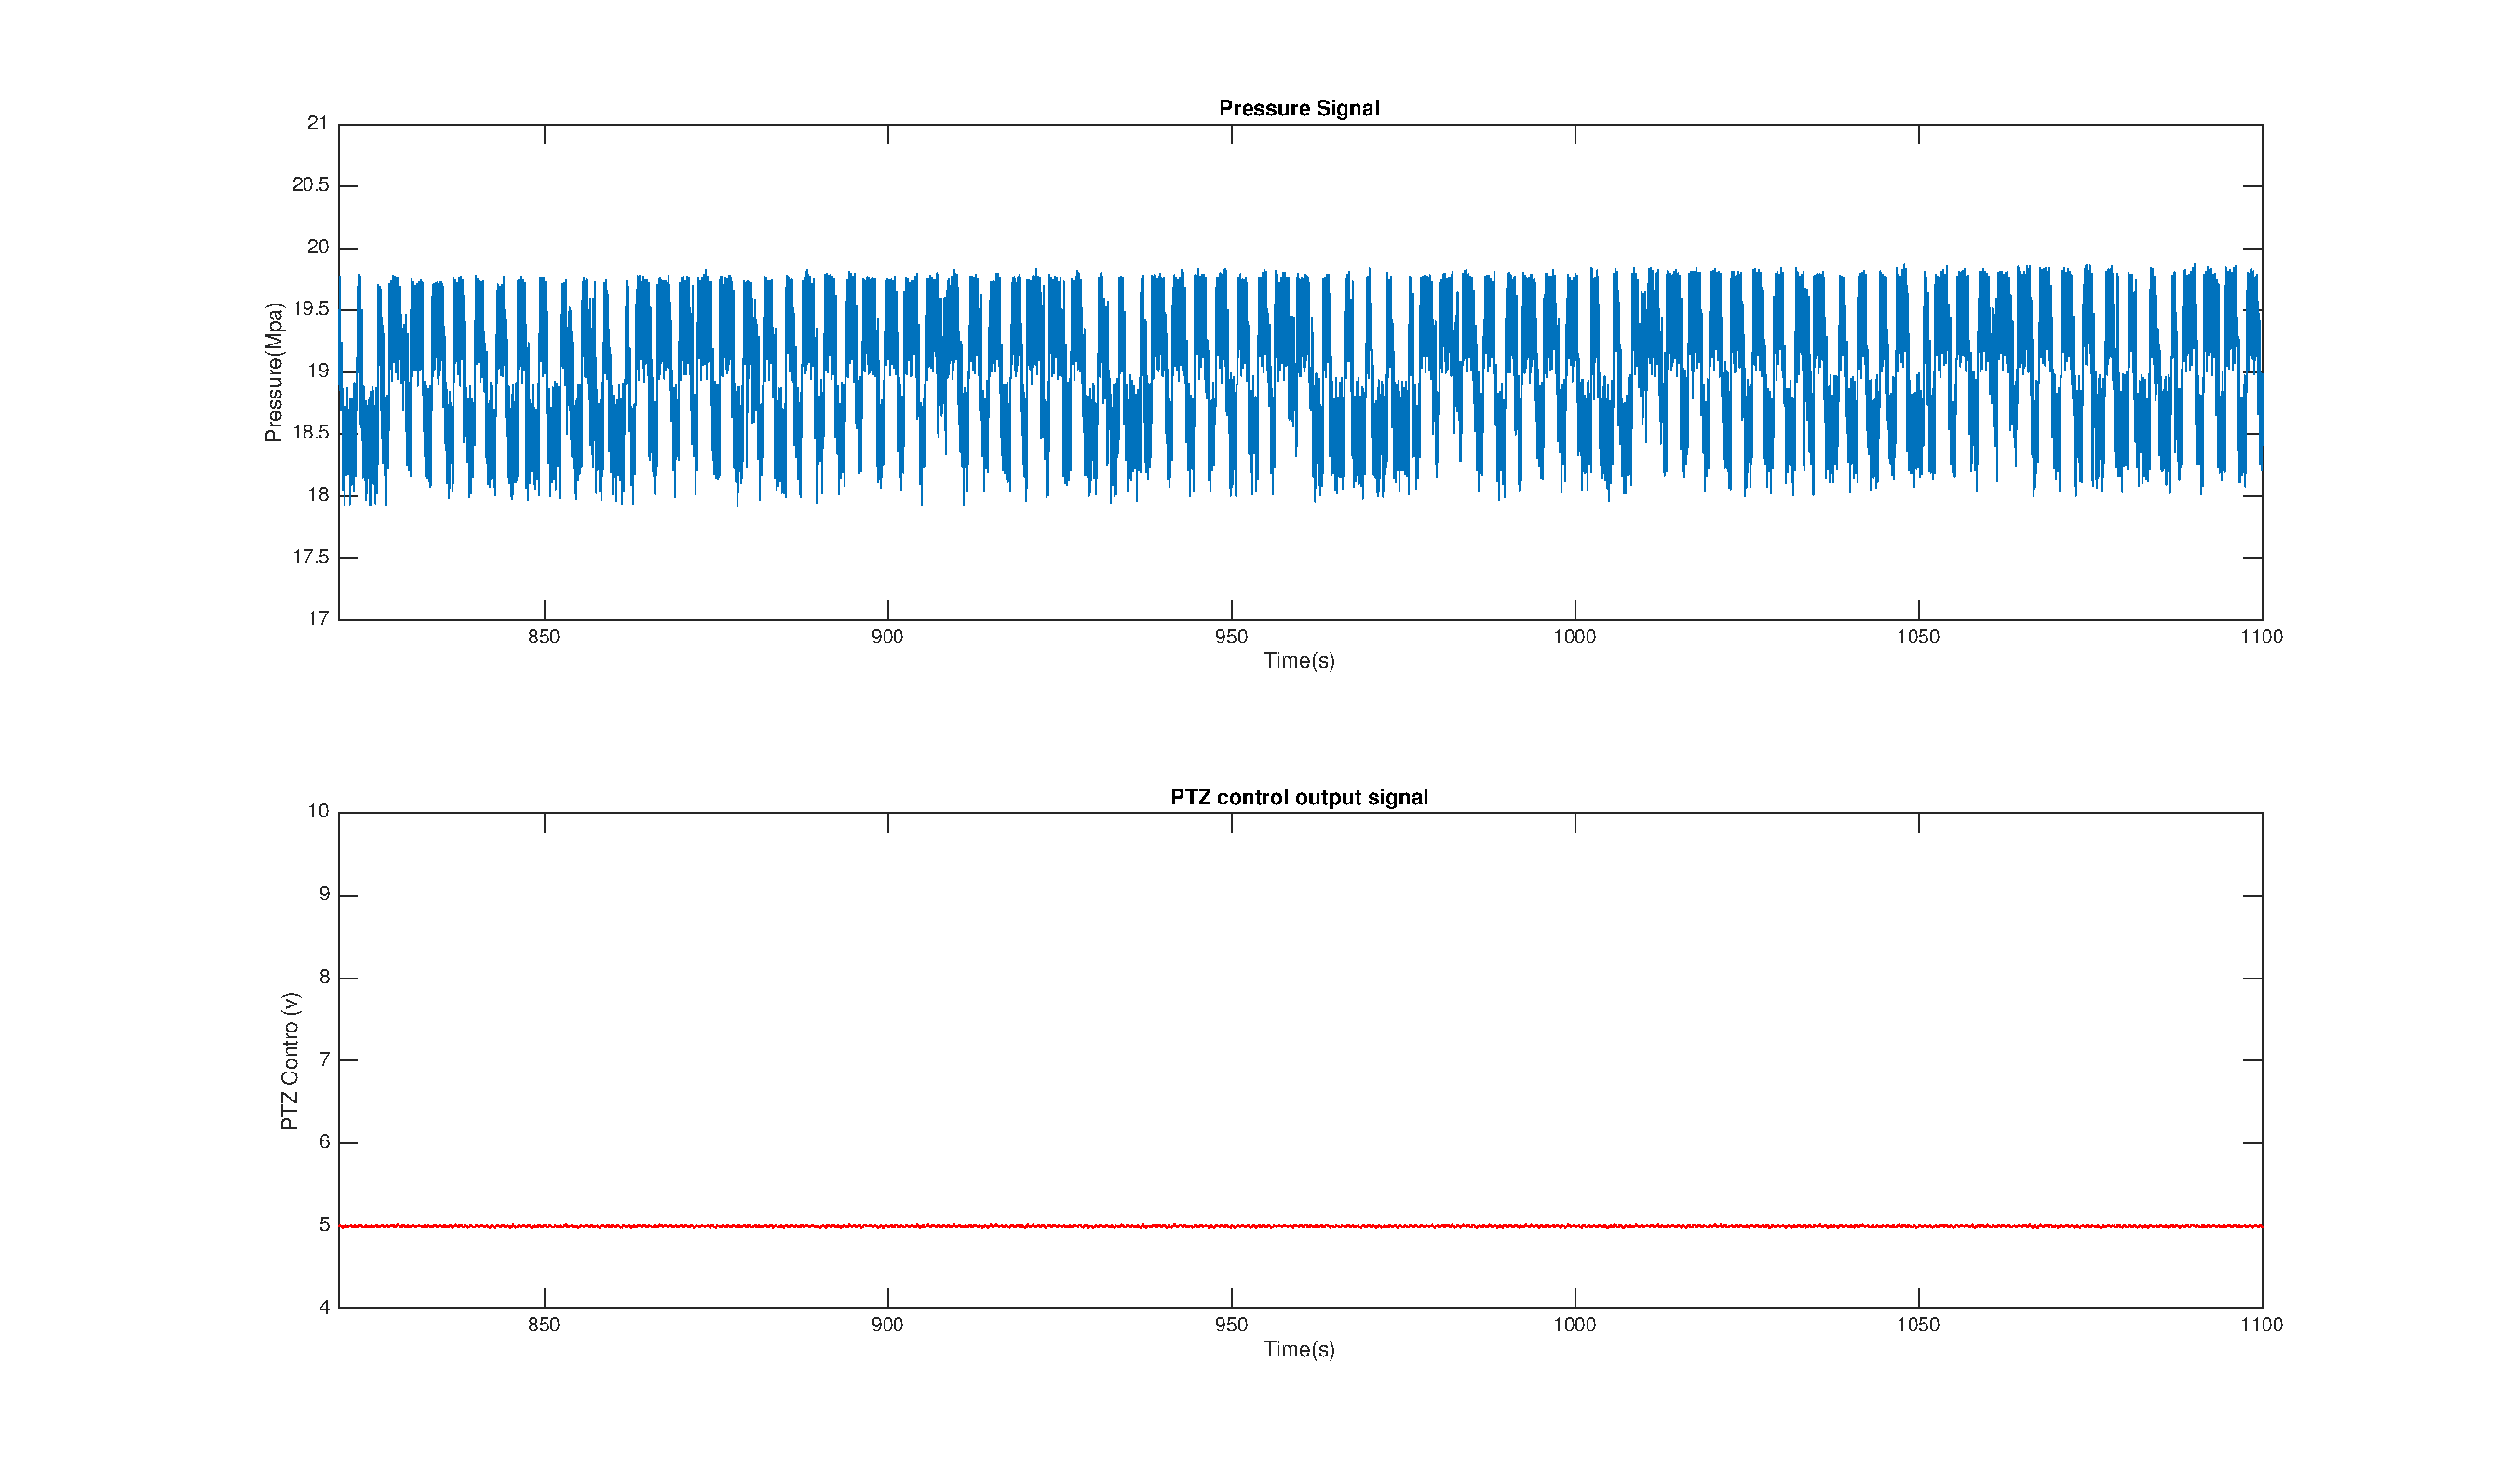
\includegraphics[width=0.9\linewidth]{./images/time_domain_result_giveup_control.eps}
\caption{停止控制之后压力脉动时域图}
\label{fig:fig12}
\end{center}
\end{figure}

\begin{figure}[H]
\begin{center}
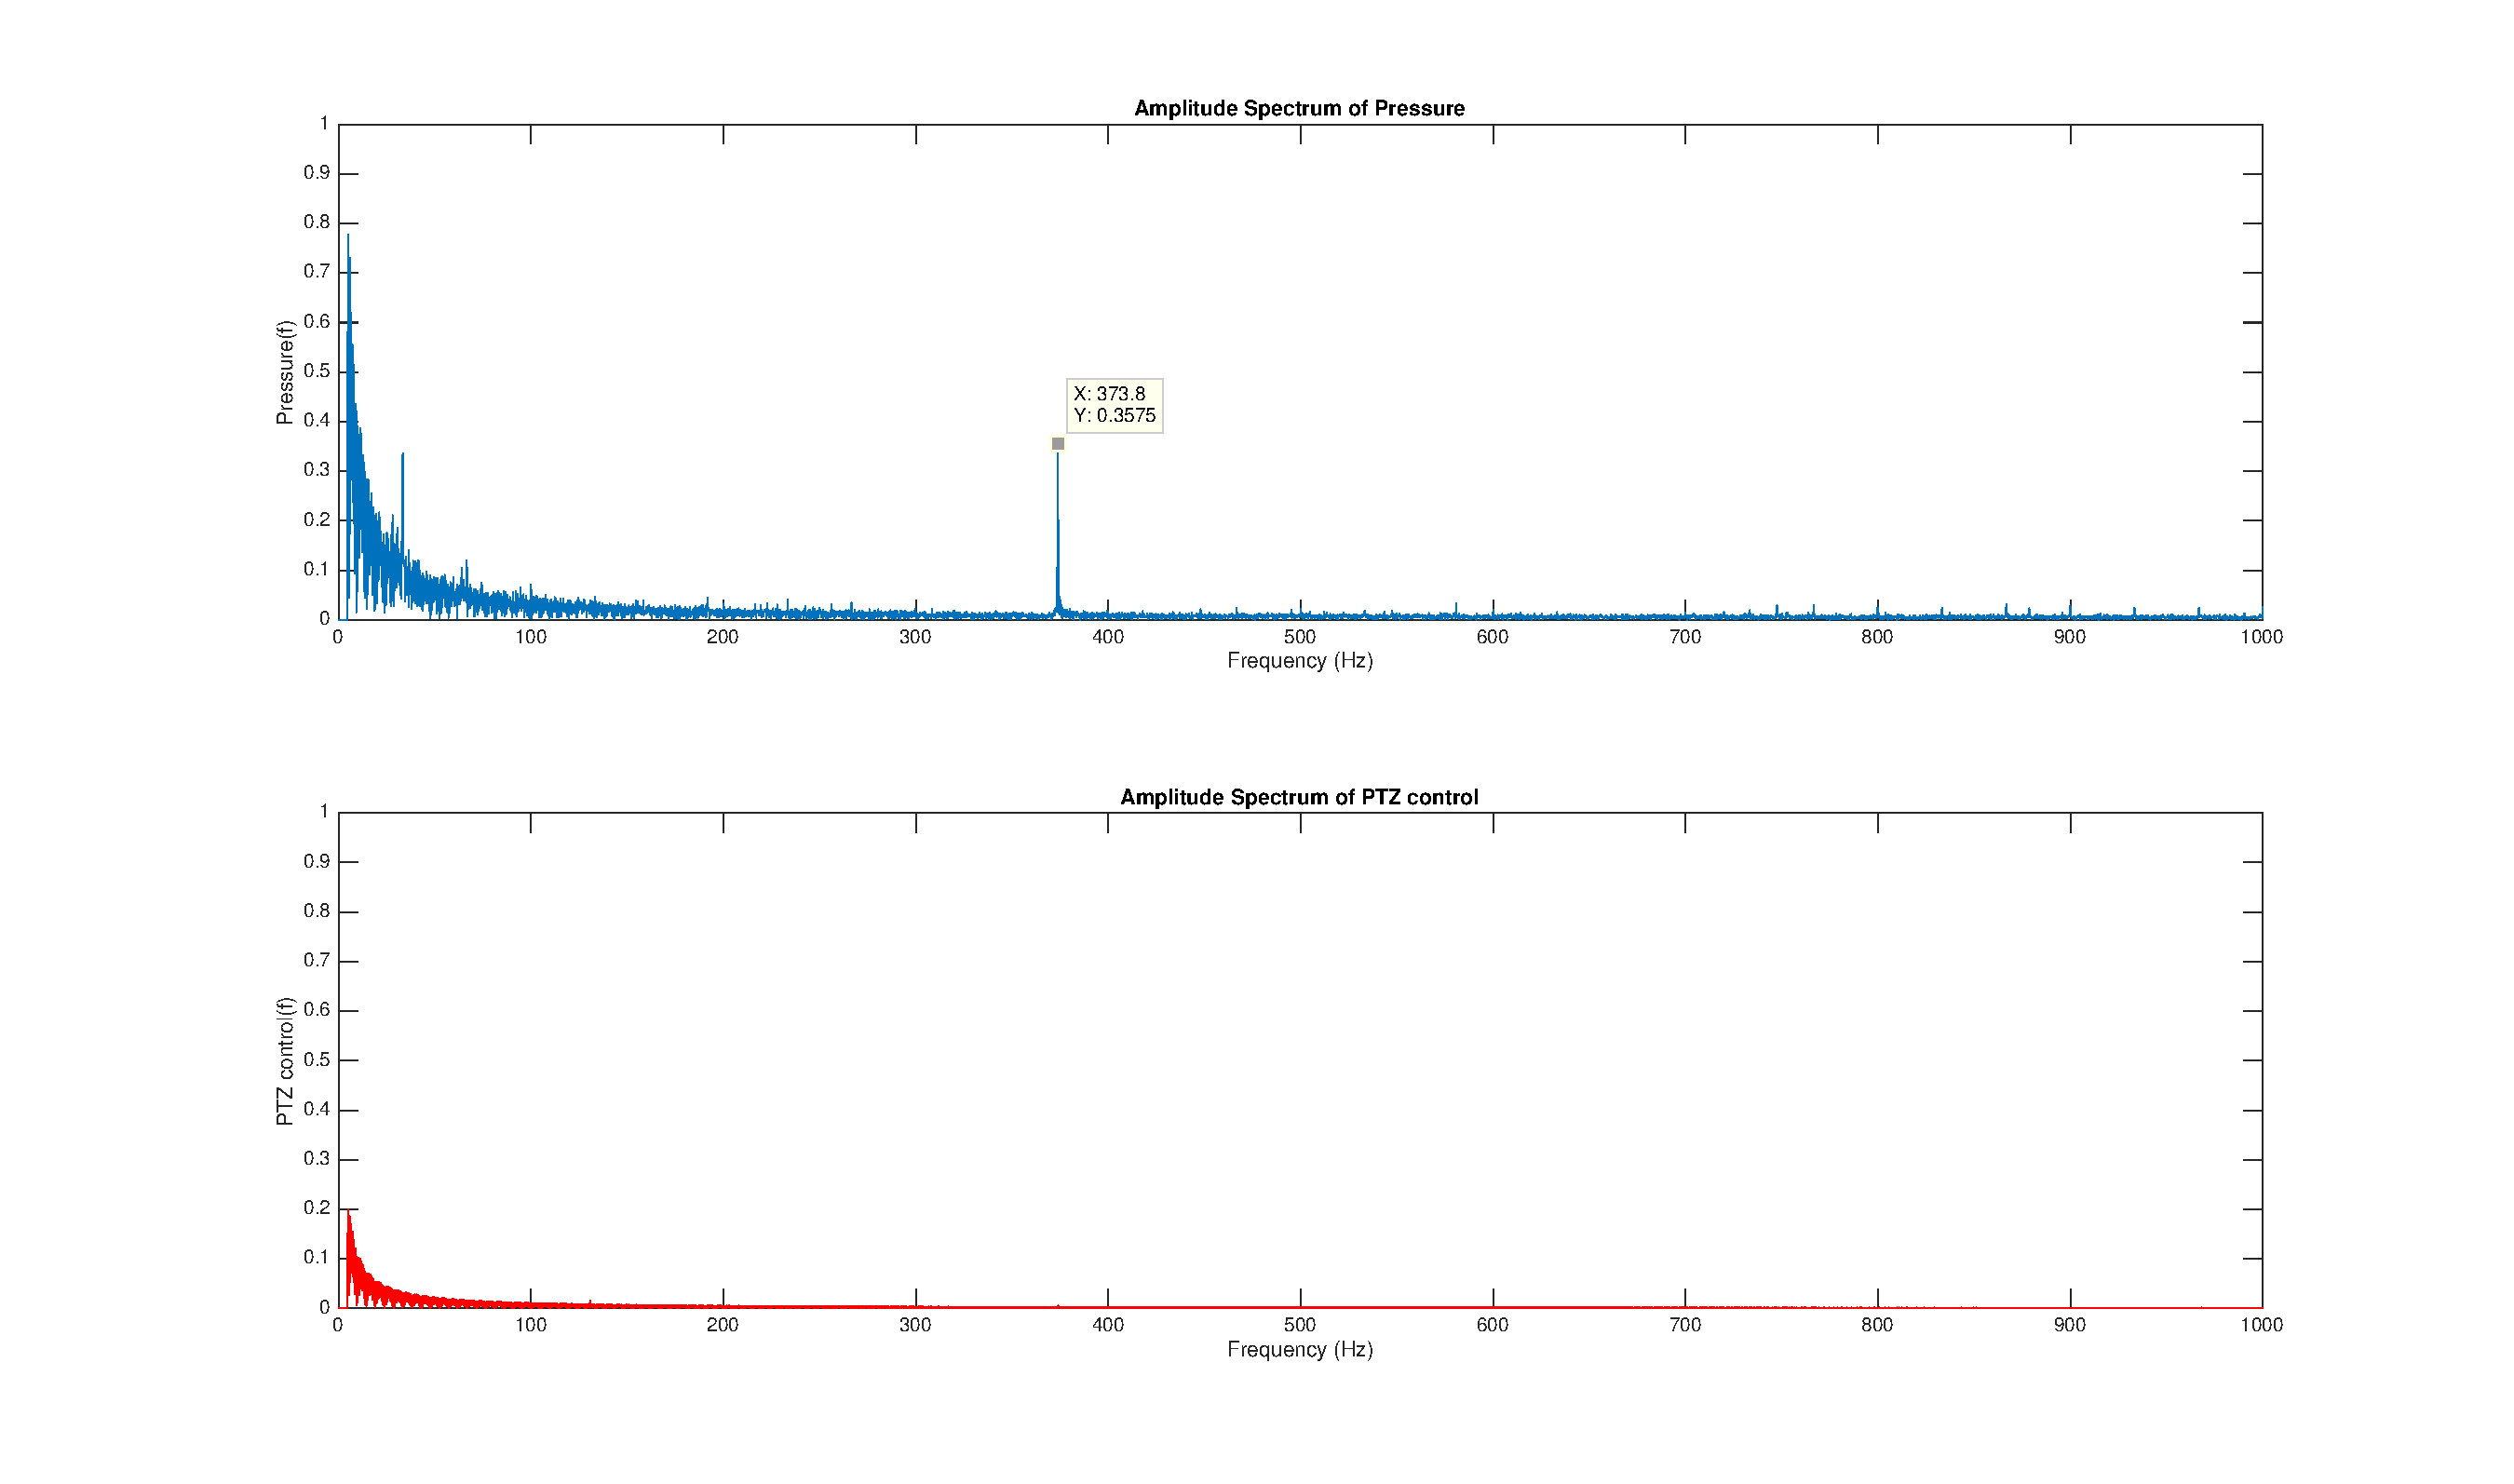
\includegraphics[width=0.9\linewidth]{./images/fft_result_giveup_control.eps}
\caption{停止控制之后压力脉动频域图}
\label{fig:fig13}
\end{center}
\end{figure}

可见,停止主动控制之后,泵的脉动又恢复了正常状态,达到了0.3575Mpa.

\subsection{施加控制相位分析}

\begin{figure}[H]
\begin{center}
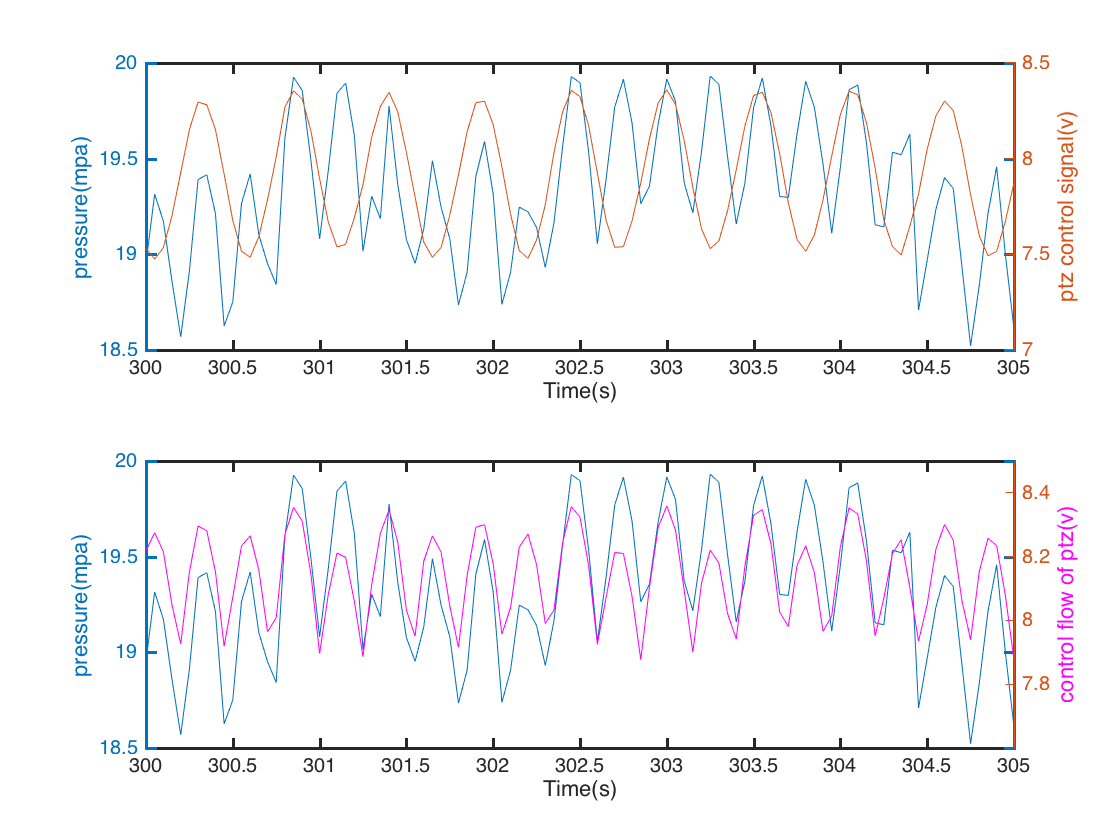
\includegraphics[width=0.9\linewidth]{./images/difference_in_plase_between_controlsignal_and_pressure.png}
\caption{施加控制压力脉动和控制信号对比图}
\label{fig:fig14}
\end{center}
\end{figure}

如图\ref{fig:fig14}所示,蓝线表示施加控制时的管路流体压力脉动,橙线表示阀芯位移指令,红线定性表示双边溢流阀的溢流流量。可见蓝线的
\subsection{进一步分析}
泵本身的稳态压力并不稳定,在小范围内存在一定程度的跳变,从图中可以看出在500s左右泵的压力发生了跳变,但并不影响算法的消振,可见算法对压力的变化有一定的容忍性,鲁棒性较强。

\section{结论}
流体管路的振动属于窄频振动,可以用自适应陷波算法框架下的自适应陷波算法进行解决。实验表明,从频域角度看,单频消振,消振效果可以达到25\%,而从时域角度看,在所有频段内,总消振效果可以达到38\%。

\section{附录}
图\ref{fig:fig15}是双边溢流主动消振实验场景图。
\begin{figure}[H]
\begin{center}
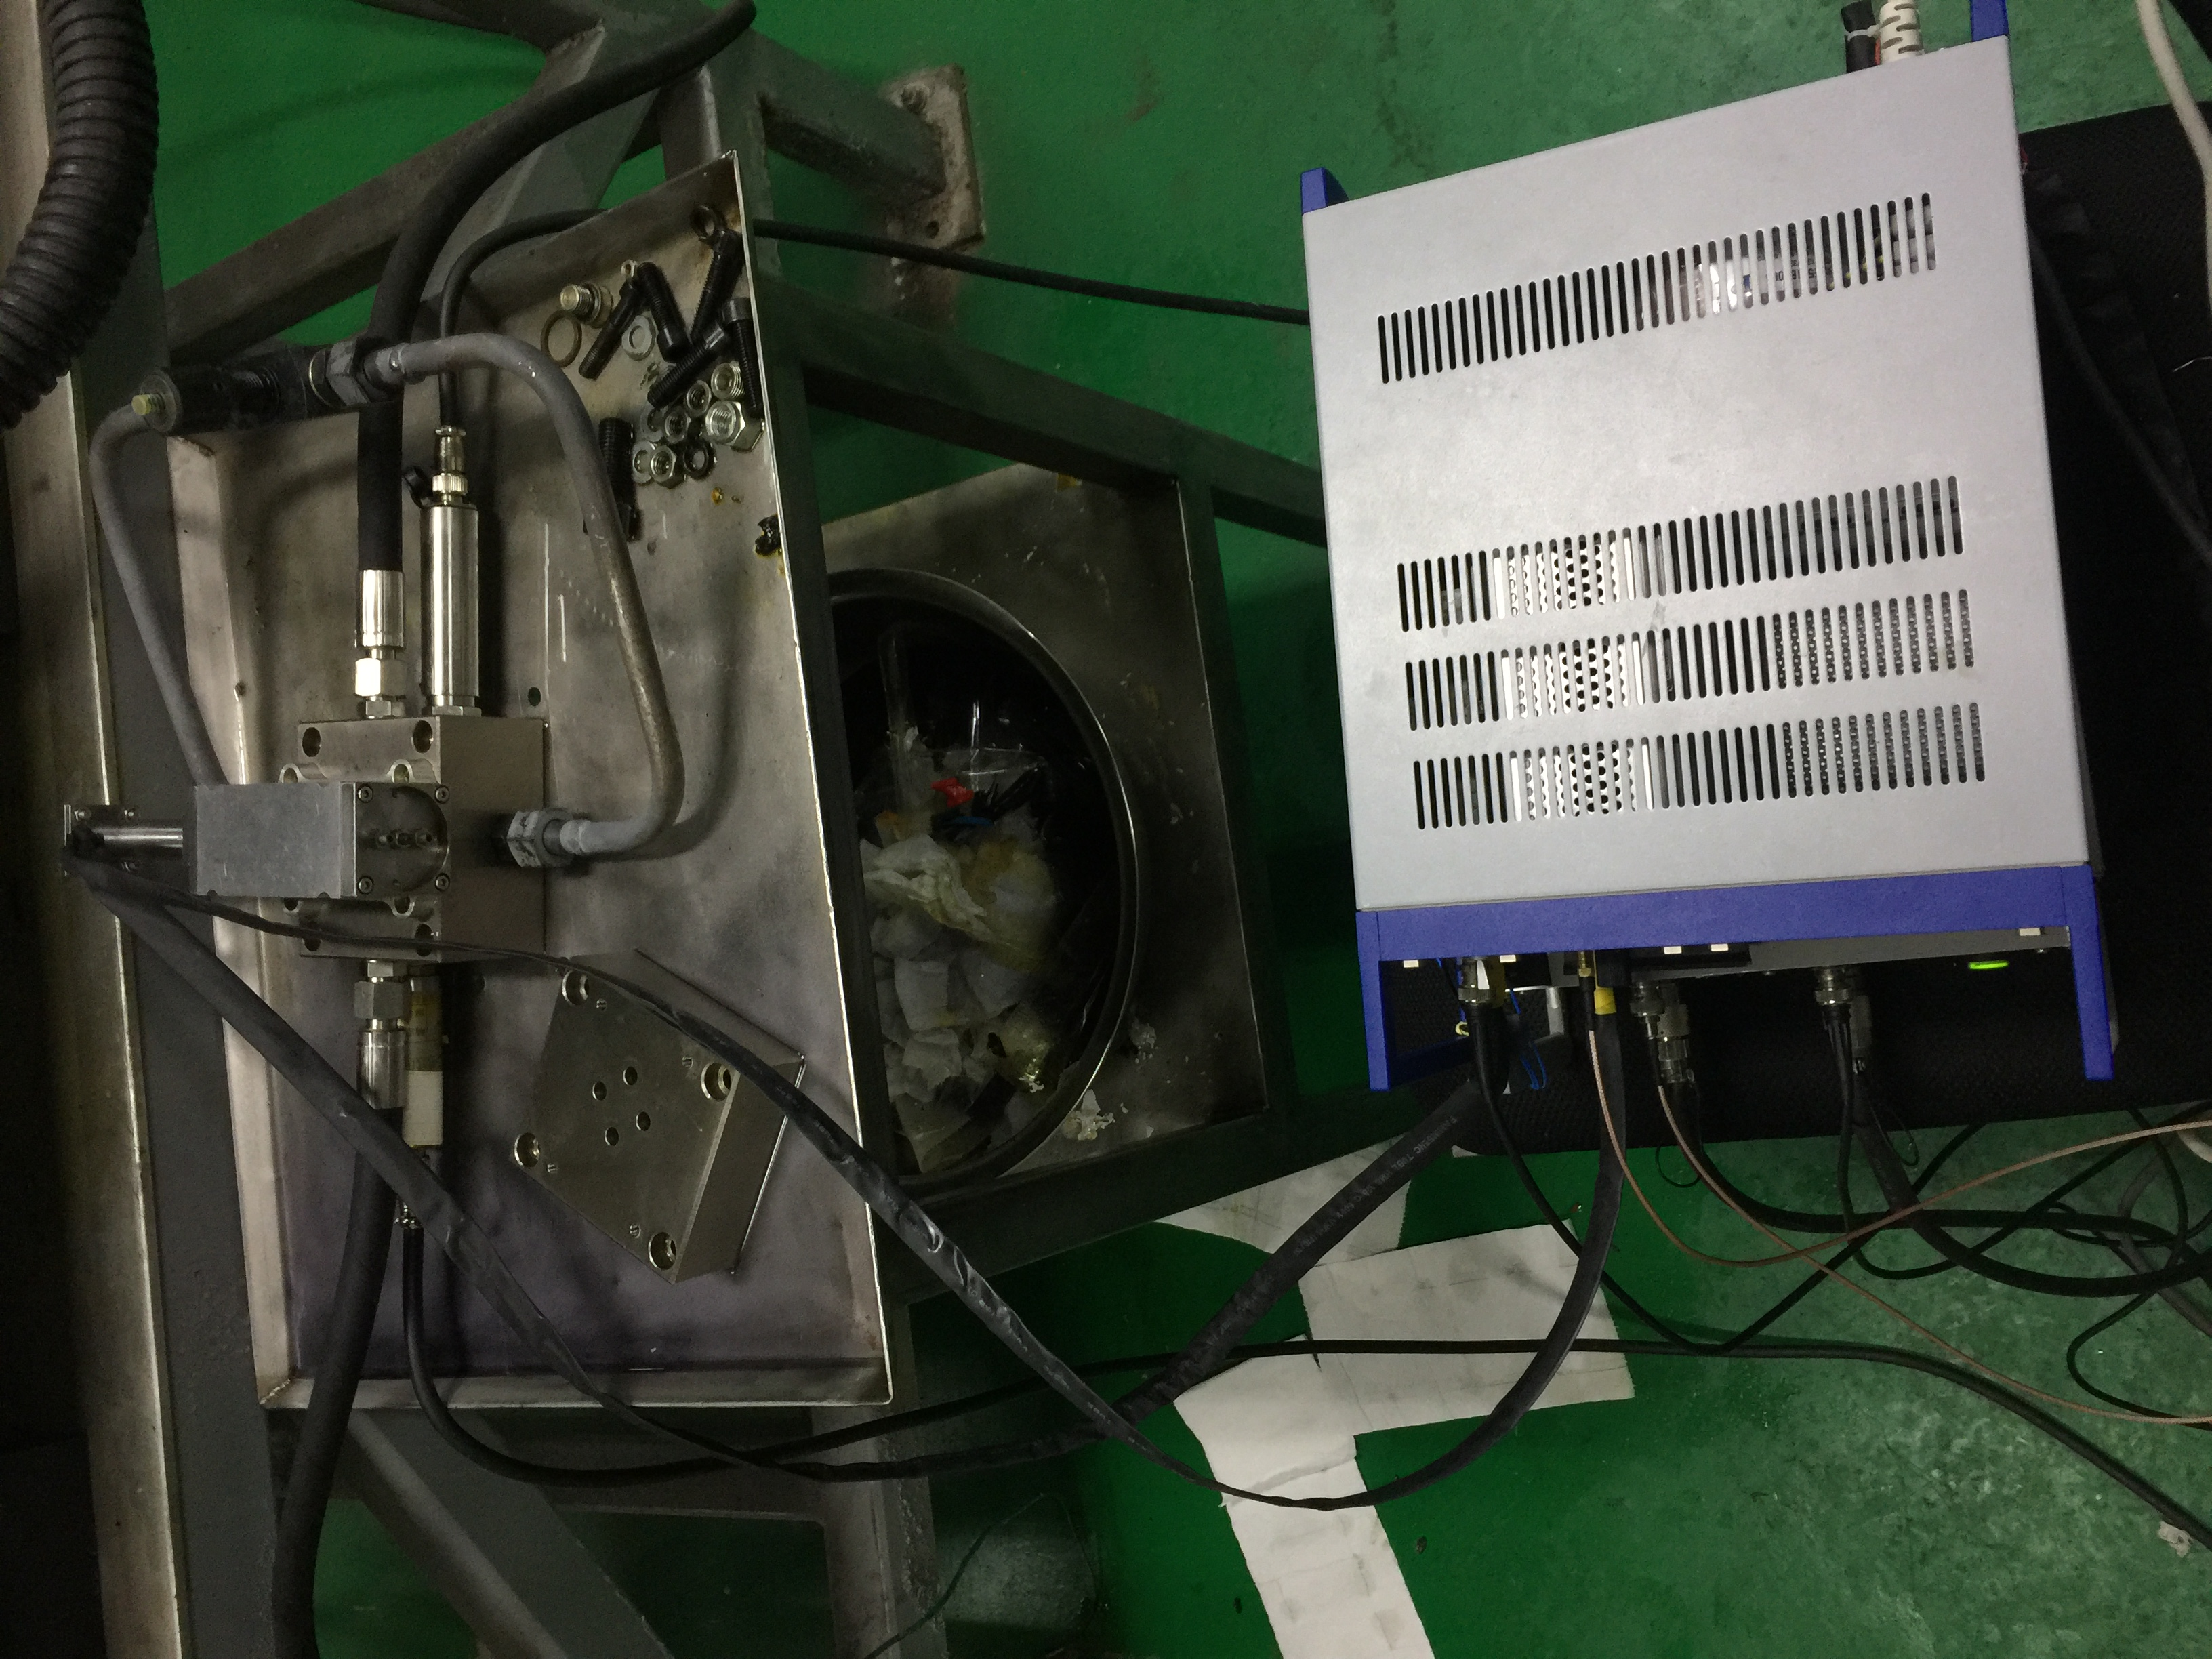
\includegraphics[width=0.9\linewidth]{./images/实验场景图.JPG}
\caption{双边溢流主动消振实验场景图}
\label{fig:fig15}
\end{center}
\end{figure}

图\ref{fig:fig16}是双边溢流主动消振系统接线图。
\begin{figure}[H]
\begin{center}
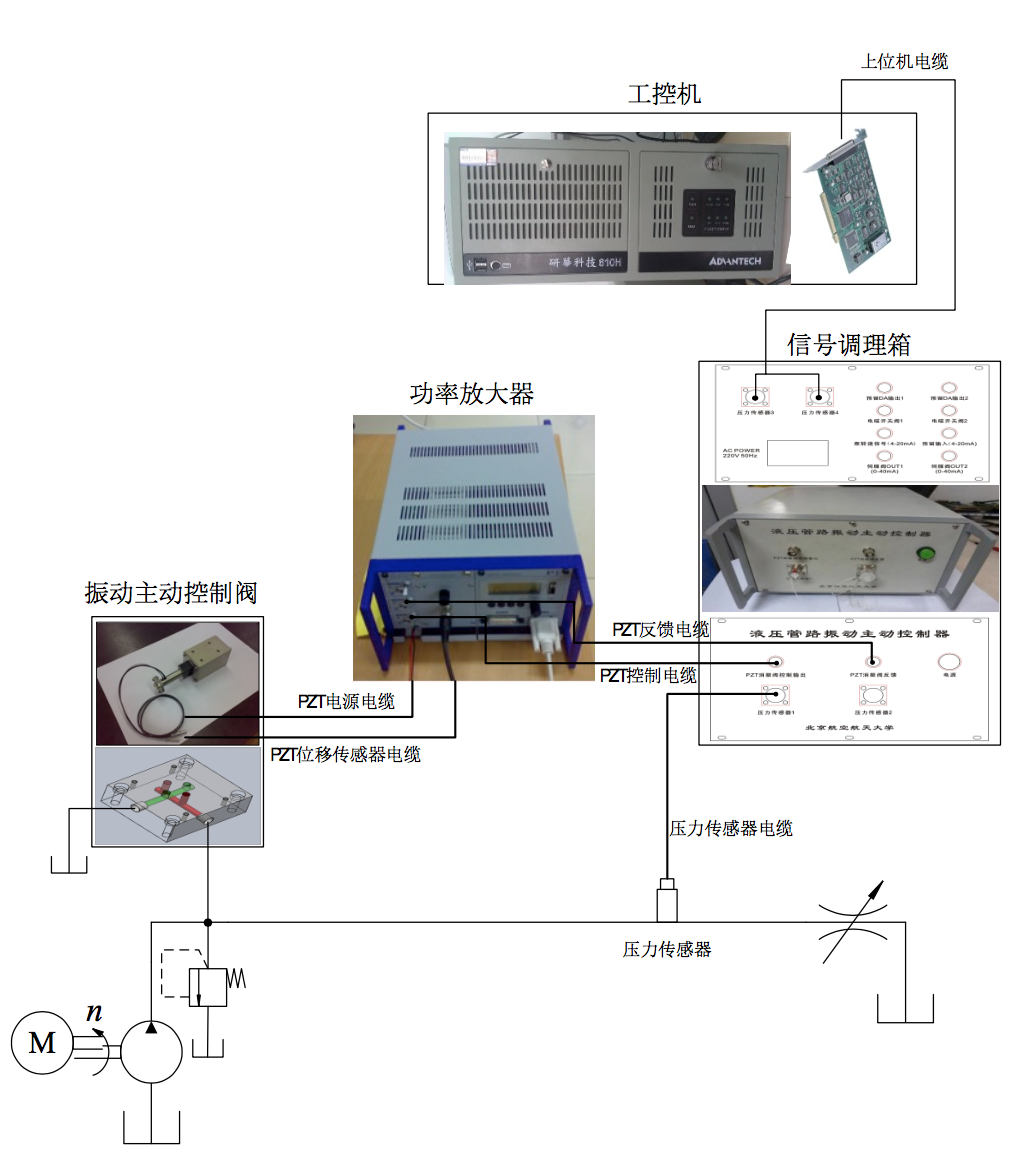
\includegraphics[width=0.9\linewidth]{./images/系统接线图.png}
\caption{双边溢流主动消振系统接线图}
\label{fig:fig16}
\end{center}
\end{figure}

%----------------------------------------------------------------------------------------
%	引用
%----------------------------------------------------------------------------------------
\newpage
{\small
\bibliographystyle{IEEEtran}
\bibliography{references}
}

\end{document}